\documentclass[12pt]{report}
\usepackage{amsmath}
\usepackage{amssymb}
\usepackage{graphicx}
\usepackage{hyperref}
\usepackage{color}
\usepackage{float}
\begin{document}
	
	\title{Chromatin Architecture Post UVC damage}
	\maketitle
	\section{Experimental Settings and Main Findings}
	\begin{enumerate}
		\item Cell type used: U20S, which are human osteosarcoma cells;
		\item H3.3 histones are tagged 48 hours before experiments using the SNAP-tag method, tag color is red;
		\item Repair factors XFP are labeled with GFP;
		\item A region of $20 \mu m^2$ was photo-activated 8-10 hours before UVC;
		\item UVC damage is induced in a region of the cell using a 266 $nm$ laser (0.266 $\mu m$);
		\item Changed to the red fluorescence signal were measured in the entire volume of the cell, post UVC;
		\item Images were acquired using confocal microscopy, with an auto-focus module on, to acquire images from the best focal plane;
		\item Fluorescence intensity were normalized against values measured in undamaged nucleus;
		\item Fluorescence loss at irradiated sites was determined by dividing the intensity in the illuminated area by the intensity of the entire nucleus after background subtraction;
		\item Illuminated area was defined 15 minutes post UVC based on GFP labeled repair factors and was kept similar throughout measurements;
		\item Fluorescent recovery was measured relative to previous illumination starting from the frame with the minimal fluorescent values;
		\item 2D projection of the 3D images were obtained by \textit{maximal intensity z projection};
		\item To gain sensitivity, most of the cell H3.3 fluorescence was photo-bleached, aside from the region of UVC illumination;
		\item 20\% loss of H3.3 signal from the \textit{entire nucleus} was detected after photo-bleaching the fluorescence patch;
		\item However, using UVC in the fluorescent patch led to 40\% loss of parental H3.3 signal, while no detectable loss was seen in the entire nucleus;
		\item The depletion of fluorescence signal in the center of the damage area, 15 minutes post UVC, was accompanied by an increase of density at its boundaries, balancing the loss;
		\item 20\% loss of DNA signal in the damage region, accompanied by an expansion of the region was observed 15 minutes post UVC;
		\item The expansion of the damage region depends on the dose of repair-factor;		
		\item The early repair factor DDB2 recruits histone chaperons HIRA, which promotes the deposition of newly synthesized histones at UVC sites;
		\item newly synthesized histones are detectable in the repair region only 45 minutes post UVC;
		\item Histone chaperons do not participate in histone redistribution after UVC irradiation;
		
	\end{enumerate}
	
	\section{Model and Parameter Estimation}
	For reasons of convenience we will work in units of $100 nm$. Parameter values calculated in the subsection below will be converted to this measure when simulated. 
	
	\subsection{Nucleus Size}
	 Cells' cross-section are 240 $\mu m^2$ in the $x-y$ plane and $11 \mu m$ in height, giving an average radius of $r_c=7.25 \mu m$.  \ref{fig:histoneMarkBeforeDamage}), The red fluorescence represent the histones.
		\begin{figure}[H]
			\centering
			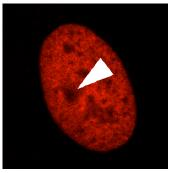
\includegraphics[width=0.2\linewidth]{../histoneMarkBeforeDamage}
			\caption{white triangle represents the UVC damage site, Histones are marked with red}
			\label{fig:histoneMarkBeforeDamage}
		\end{figure}
		
	\subsection{The Simulation Domain}
	We set our simulation in a spherical domain with reflecting boundaries. This $d$-dimensional sphere, $\Omega_d(\rho)$ of radius $\rho$, will represent a region around the damage site, rather than the entire nucleus. 
	To keep the polymer dense inside this region, we set $\rho=(b\sqrt{N/6})/2$. The actual value of this parameter is yet to be justified. The reflecting boundaries mimic the condensation barrier of the DNA with surrounding chromosomal chain, unaffected by the UV damage. 
		
	\subsection{The UV beam}
	UV beam has 3 $\mu m^2$ section, yielding a radius of $r_{uv}=\sqrt{\frac{3}{\pi}}\approx 1 \mu m$. 
	In simulations we set the beam radius to be proportional to the polymer's radius of gyration, such that the simulation domain is 3 times the radius of the UVC beam. We therefore set the UVC beam radius, $\rho_B$, to be  
    $\rho_B=\rho/3=(b\sqrt{N/6})/6$.
	
	\subsection{The region of interest (ROI)}
     The area of chromatin expanded after UVC occupies $10 \mu m^2$ which gives 3 times the UVC beam radius, i.e. $3\mu m$. In practice, we define the ROI as a rectangular region with diagonal $\rho_R$, proportional to the UCV beam's radius. The ROI's vertexes lay on the boundary of $\Omega(\rho)$, allowing room for monomers outside the ROI after expansion. 
		
    \subsection{Histone Density}
		We consider histones to be uniformly distributed in the nucleus and in the damage zone. There are $3\times 10^6$ histones marked, which makes their density $3\times 10^6 /(4 \pi 7.25^3)\approx 630$ histones/$\mu m^3$
		The expected number of histones in the UV beam region is $14.5\pi \times 630\approx 30,000$ histones, assuming the beam is shot through the center of the sphere. 
    
    \subsection{DNA density}
	to be determined	
	
	\subsection{Distribution of damage sites}
	to be determined
	
				    
	\subsection{The chromatin}	
     The chromatin is modeled as a Rouse polymer of $N$ monomers connected by harmonic springs. The dynamics of the polymer is governed by 3 forces: thermal fluctuations, spring force, and bending force, which we vary during simulations to approximate the observed experimental behavior. Before UVC beam is shot the polymer dynamics is governed by spring forces only, whereas after UVC the affected monomers of the chain along with their nearest neighbors are assigned additional bending elasticity forces. 
     
     Thermal diffusion fluctuation, results from the random collision of the polymer with the particles of its surrounding, and is given by 
     \begin{equation*}
     F_d(t) = \sqrt{2D}\frac{dw}{dt}
     \end{equation*}
      with $D$ the diffusion constant, defined by $\frac{k_BT}{\xi}$, $k_B$- the Boltzmann constant, $T$- the absolute temperature in Kelvin, $\xi$-the friction coefficient, and $w$ is a standard white Gaussian noise. 
            
     The spring force, derived from an harmonic potential of springs connecting neighboring monomers, is given by
     \begin{equation*}
      F_e(t) = -\gamma_e\frac{dk_BT}{2b^2}\frac{\partial}{\partial R_n}\sum_{n-1}^{N-1}(|R_n(t)-R_{n+1}(t)| -l_0)^2
     \end{equation*}
     with $\gamma_e>0$ spring constant,$d$ is the dimension, $b$- the standard deviation of the distance between monomers, $R_n(t)$ is the 3D position of the $n^{th}$ monomer at time $t$, and $l_0$ is the minimal allowed distance between neighboring monomers.
     
     Bending force on the $n^{th}$ monomer is defined in terms of the angles $\theta_i$ between three adjacent monomers of the chain, $n,n+1,n+2$;
     \begin{equation*}
     F_b(R_n) = -\gamma_b\frac{dk_BT}{2b^2}\frac{\partial}{\partial R_n}\sum_{i=1}^{N-2}(\cos(\theta_i(t))-\cos(\theta_0))^2
     \end{equation*}
               
     The differential equation describing of motion of the chain is thus 
     \begin{equation*}
     \frac{dR_n(t)}{dt}= F_e +F_b +\sqrt{2D} \frac{dw}{dt}     
     \end{equation*}
     
    \subsection{Model Parameters}
      Parameters used in simulations are set proportional to of the quantity $\frac{dk_BT}{b^2}$, which we fix to be 1 by setting the friction factor $\xi=1$. 
    \subsubsection{The parameter b} 
      we set $b=\sqrt{dimension} \times 100 nm$, 
    \subsection{The minimal distance between monomers -$l_0$}
     We set $l_0$ to be $\sqrt{d}$ to match $b$ and allow fast relaxation of the chain configuration before UVC beam shot, after diffusion is turned off. 
    \subsubsection{Number of monomers}
      The number of monomers, $N$, is determined by setting the polymer's radius of gyration to covers the ROI. The radius of gyration is given by $\sqrt{N/6}b$, equating it to $3\mu m$ we get $N\approx 1800$                      
     \subsubsection{The Spring constant}
       We set the spring constant $\gamma_s =1$
     \subsubsection{The bending constant}       
       The bending constant was observed to affect the rate at which the polymer assumes new conformation after UVC damage.
       We set it to be proportional to the bending constant, as $\gamma_b frac{3K_bT}{b^2}$. later we will adjust this constant according to the rate of chromatin expansion seen in experimental data. 
             
      \subsection{UVC damage effect on monomers}
       We assign bending elasticity to affected monomers, with an opening angle $\theta$ (see Parameters section). Through experiments we have observed that in many cases there were affected monomers with no neighboring affected monomers. This isolated affected monomers' dynamics was observed to be not ordinary after assigning them bending elasticity. We, therefore, assign bending elasticity force also to their nearest neighbors to prevent these phenomenas and to form a more continuous segments affected by bending. 
       
     \subsection{Affected monomers after UVC}\label{subsection_affectedMonomersAfterUVC}
     Affected monomers are those found within the UVC beam at its initiation. The probability of a monomer to be damaged follows a Gaussian distribution with its center at the UVC beam's center-of- mass, which is placed at the polymer's center-of-mass at the moment of UVC beam shot.       
      
    \subsection{The ROI}
    The circular region of interest (ROI), in which we calculate monomer densities gain and loss, is determined according to the expansion of the damaged monomers.
    We set the percentage of included damaged monomers to 95\%. The ROI is calculated from the polymer's center-of-mass, such that 95\% of the damaged monomers are included within it. 
    The ROI is calculated at the end of the repair phase, after expansion has thought to reach saturation [How is saturation determined?]. The radius of the ROI is then used to back-calculate the densities within it relative to the center of mass of the polymer at any time step starting from the beam shot time. 
    \subsubsection{determining expansion saturation}
     In the current version of the simulation framework, we assume the expansion of the affected monomers has reached saturation at the end of repair phase. To determine the radius of the ROI, we take the average of the affected monomers' radius of expansion in the last 10\% of the steps in the repair phase. 

    		             		
	\section{Simulations}	
	
	\subsection{Simulations' settings}
	Simulations were ran $numRelaxationSteps$ up to relaxation, after which the diffusion force was set to $0$ and recording for $numRecordingSteps$. Following, the UV beam was shot through the center of the polymers mass. Monomers found within the UV beam area were assigned bending force with a probability following a Gaussian distribution. To prevent out-of-the-ordinary monomer behavior, we assign bending force to the affected monomers' nearest neighbor along the chain (see subsection \ref{subsection_affectedMonomersAfterUVC}). Nearest neighbors were not counted as affected monomers. Simulation then ran for additional $numBeamSteps$ with the bending force active for the affected monomers.
	
	Simulation were placed in a spherical domain with reflecting boundaries.
	Measurement of density were performed on a circular region, with its center dynamically placed at the polymer's center-of-mass, and it's radius determined at the end of the repair phase.
	Sizes of the containing sphere (circle in 2d) and the measurement region were proportional to the radius of gyration, $\sqrt{N/6}b$.
	
	\section{3D Simulations}
	 \subsection{The number of monomers in the ROI as a function of the bending constant}
	  In this experiment we examine the affect of the value of bending/spring constants on the number of monomers left at the ROI post UVC. 
	  For this end we examine 5 different type of chains, with number of monomers,$N$ varying as $N=100, 200, 400, 800,1600$. For each $N$ we keep the spring constant,$\gamma_s=1$, and increase the bending constant $\gamma_b= 1,2,3,4,5$. For this simple experiment we perform only one realization per chain per bending constant, hence the results presented in the following table should be interpreted  with care. 
	  \underline{Parmeter used in simulations}:
	  
	  \begin{itemize}
	  	\item \textit{numRelaxationSteps} = 2000
	  	\item numRecordingSteps  = 1000
	  	\item numBeamSteps       = 3000
	  	\item numBeads = [100 200 400 800 1600]
	  	\item dt       = 0.1
	  	\item D        = 1;
	  	\item b        = $\sqrt{3}$
	  	\item opening angle $\theta_0$ = $\pi$
	  	\item bending constant = $[dD/b^2, 2dD/b^2,3dD/b^2,4dD/b^2, 5dD/b^2]$
	  	\item springConstant   = $dD/b^2$
	  	\item beamRadius = $\sqrt{numBeads/6}b/6$
	  	\item containingSphereRadius = $0.5\sqrt{numBeads/6}b$
	  	\item regionOfInterestWidth  = $2(\sqrt{numBeads/6}b)/6$
	  	\item regionOfInterestHeight = $2(\sqrt{numBeads/6}b)/6$
	  	\item regionOfInterestCenter = polymer center of mass
	  \end{itemize}
	  
	 
	  \begin{table}[H]
	  	\tiny{
	  		\begin{tabular}{c| l l l l l}
	  			&           & & Lost (mean) (\%)[min max]& &  \\
	  			\hline
	  			&           & & bending const. multiplier. $\gamma_b$ & &  \\
	  			\hline 
	  			$N$ 	   &            1 & 2 & 3 & 4& 5 \\   	 
	  			\hline 
	  			100 & 31 (58\%) [28,38] & 35 (16\%)[-3 17]    & 14 (37\%) [11 22] & 36 (61\%)[26 43]   & 10 (26\%)[2 26]\\
	  			200 & 17 (21\%) [2, 30] & 58 (57\%)[49 71]    & 54 (56\%)[48 62]  & 86 (72\%) [82 92]  & 33 (45\%)[28 32]\\
	  			400 & 22 (16\%) [2 39]  & 100 (53\%) [82 106] & 73 (39\%)[60 89]  & 92 (\%)[72 100]    & 117 (66\%)[74 120] \\
	  			800 &  0 (0\%) [-20 18] & 0 (0\%) [-39 29]    & 72 (20\%)[4 133]  & 122 (33\%)[29 196] & 120 (31\%)[0 180]\\
	  			1600&  0 (0\%)[-23 21]  & 0 (0 \%) [-47 25]   & 54 (9\%)[0 104]   & 43 (3\%)[-17 110]  & 67 (12\%)[0 132]\\
	  		\end{tabular}
	  	}
	  \end{table}
	  
	\section{2D simulations}
		
		
	\subsection{Adding Lennard-Jones force to stop expansion}
      After UVC, several monomers are hit and together with their nearest-neighbors are assigned bending elasticity with an opening angle of a certain value. Usually, a region of consecutive affected monomers is enclosed by non-affected monomers. Therefore, the result of activating the bending elasticity force for the affected monomers is the formation of horse-show type of loops structures. 
      Affected monomers are located at the center of the polymer and expand usually outwards (although the direction of expansion cannot be controlled). The problem is that the expanded region of the chain exit the ROI and keep expanding passed the layer of non-affected monomers, that are usually located outside the ROI. 
      
      The Rouse polymer permits bonds to cross each other, and therefore the affected monomers do not stop at the non affected monomer layer. 
      to try to confine the affected monomers to the region of the damage, we assign volume exclusion, Lennard-Jones potential, to the chain. The non-affected monomers will hopefully counter-balance the expansion of the affected monomers, keeping them from passing the non-affected layer outside the damage zone.
      
      In the experiments explained below we ran the simulation to see if the radius of expansion of the affected monomers can be limited by the Lennard-Jones fores. Simulations are performed in two-dimensional spherical environment, the polymer includes 500 monomers.
      
      
     \begin{figure}[H]
     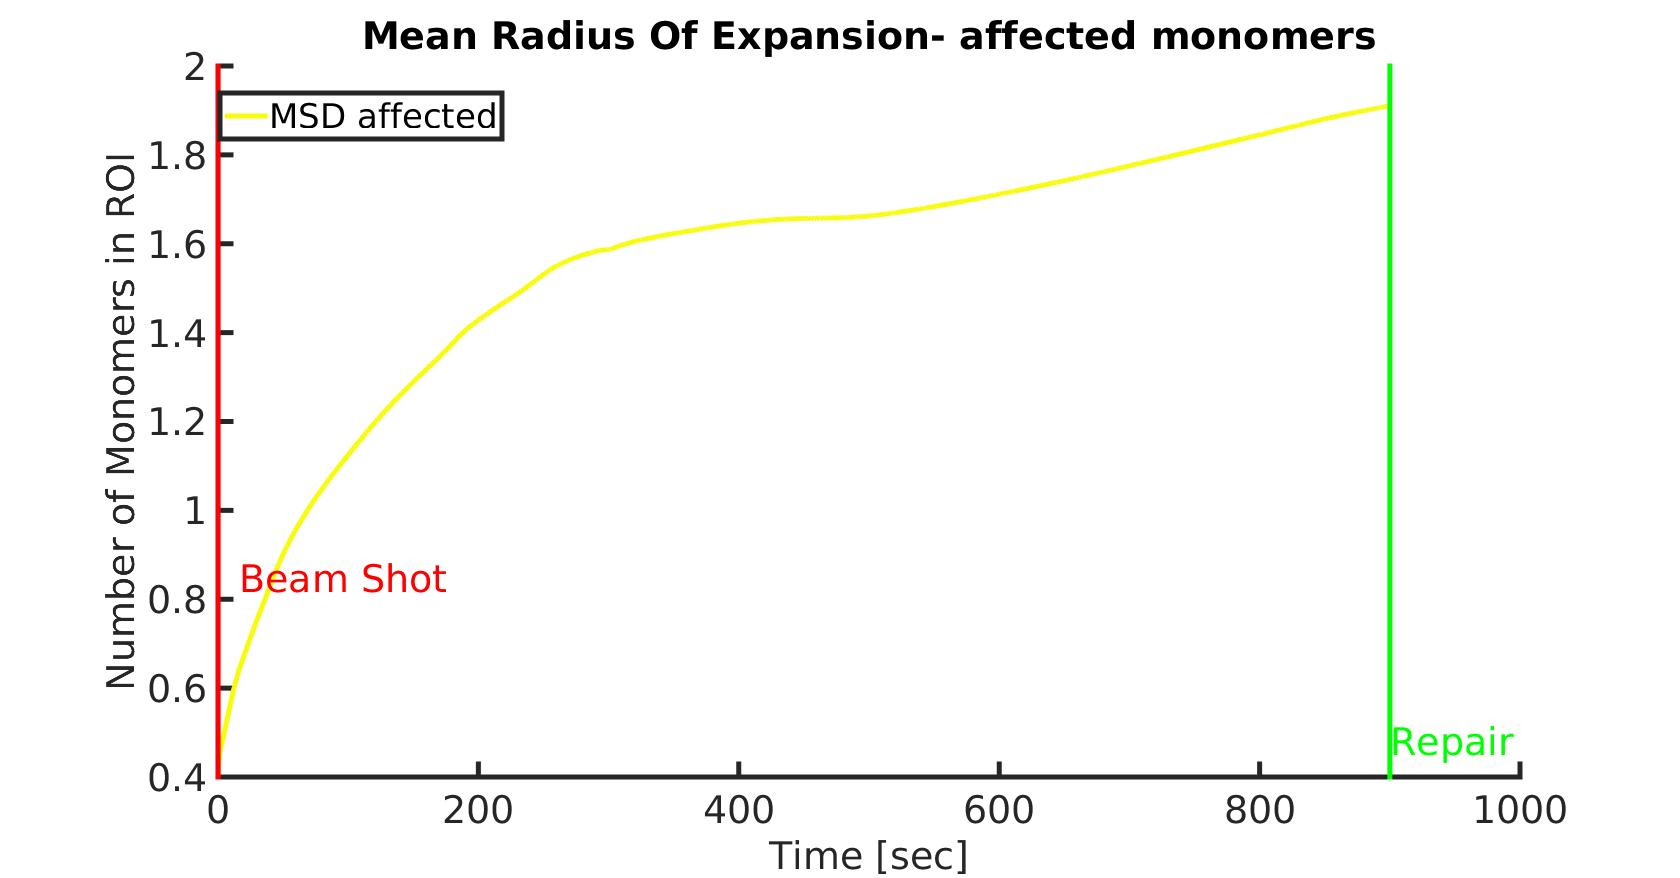
\includegraphics[width=0.5\linewidth, height=0.3\textheight]{RadiusOfExpansion500BeadsLennardJones}
    	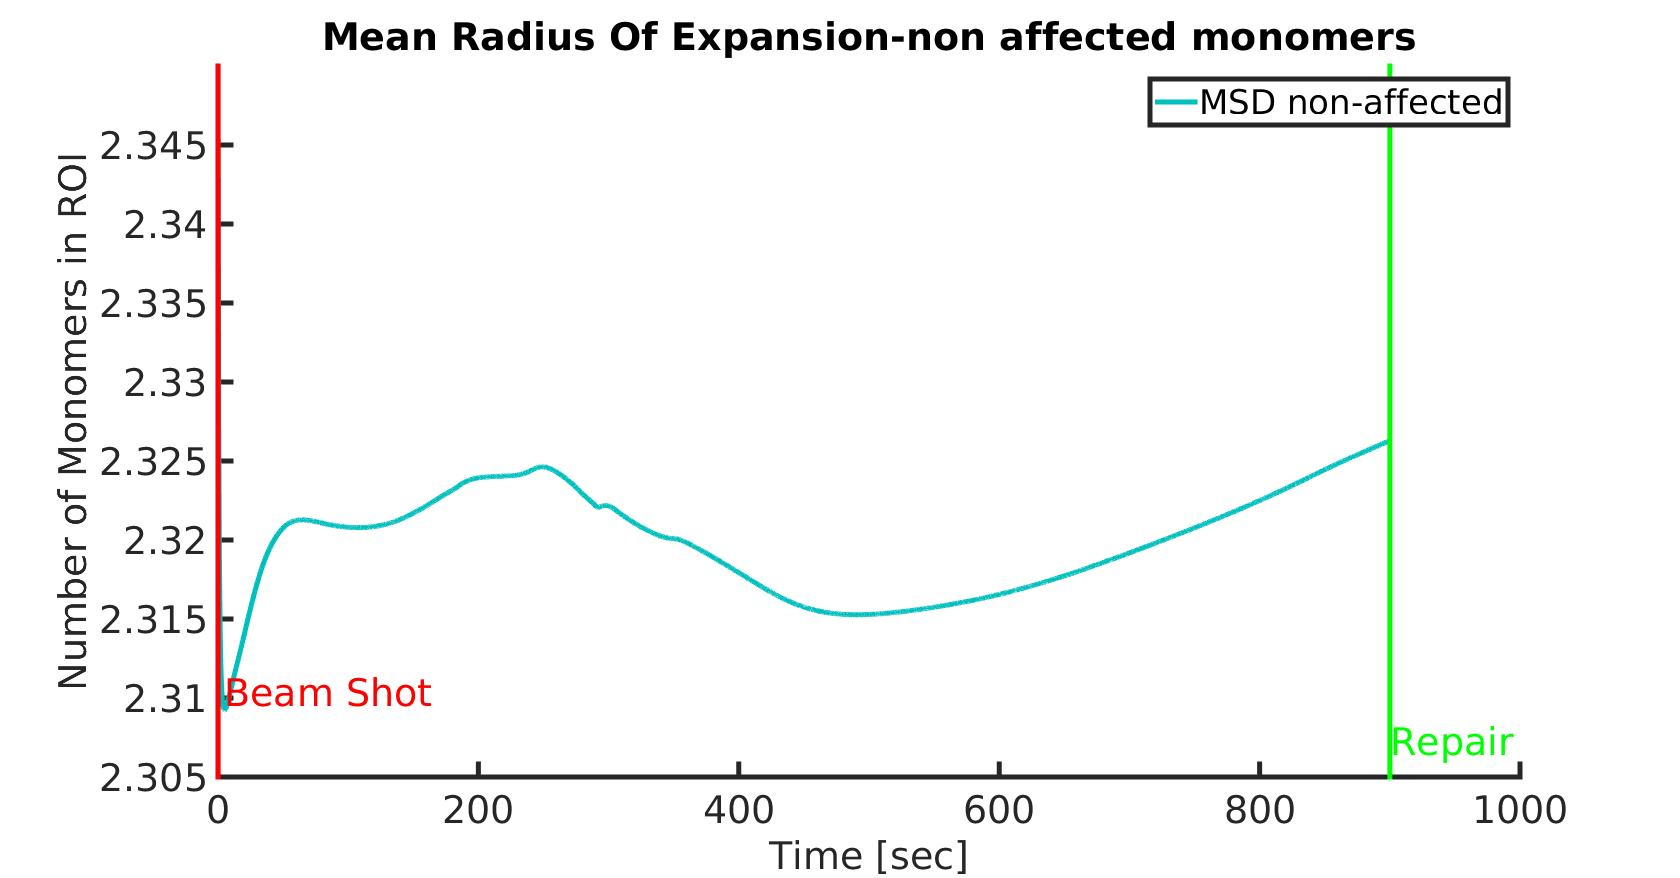
\includegraphics[width=0.5\linewidth, height=0.3\textheight]{RadiusOfExpansion500BeadsNonAffectedLennardJones}
        \caption{Radius of expansion relative to the monomers' center-of-mass, for the affected (left) and non-affected (right) monomers of the chain.(Mean of 5 experiments of 9000 steps each, polymers contain 500 monomers)}
        \label{fig:RadiusOfExpansion500BeadsLennardJones}
      \end{figure}
      
      From figure \ref{fig:RadiusOfExpansion500BeadsLennardJones} we can see that the Lennard Jones is not sufficient to stop the monomers from expanding. The affected monomers MSD keeps increasing until about time 300 sec, where it reaches a plateau. at this point many beads are at the same line as the non affected ones and probably the expansion comes into a halt. Once the bending force overcomes the resistance by the Lennard Jones force, the expansion continues. The affected beads' radius of expansion doesn't reach the value of the non affected. However, we suspect that it will given enough time. Moreover, the expansion is measured relative to the center of mass of either one of the two groups, affected and non-affected, and so it is not clear where are those two groups relative to each other. 
      
      Changing the radius of expansion to be calculated relatively to the beam center does not change the size of expansion. The affected monomers keep on expanding. 
      
      We therefore, omit the Lennard-Jones potential from further consideration.


   \subsection{Cross-linking the polymer}
	In addition to the linear backbone of the polymer, we randomly add connectors between pairs of non nearest neighbor monomers. The measure for connectivity we use is the percentage of connected pairs out of the number of monomers, e.g. 50\% connectivity in a 100 monomer chain  corresponds to 25 additional connector (connecting 50 monomers). 
	At simulation initiation, we let the polymer relax to a state in which the cross-linked monomers are brought into proximity. After UVC beam shot, we divide our results into two parts. In the first, we assign bending potential to the damaged monomers, in the second we assign bending potential to the non-damaged monomers. We further divide each case into two scenarios according to the effect of UVC. In the first, we break all cross-links connected to any affected monomers in the beam. In the second, we keep all cross-links throughout the simulation. 
	In all simulation in the subsection the ROI was determined according to the damaged monomers.
	
	\subsection{Assigning bending to damaged monomers}
	In this simulation we assign bending elasticity to damaged monomers and their nearest-neighbor. The ROI is determined by the expansion of the damaged monomers. 
	
	\subsubsection{Break damaged monomers' cross-links}
	After UVC we break all cross-links to and from any damaged monomers. 
		
	\begin{figure}[H]
	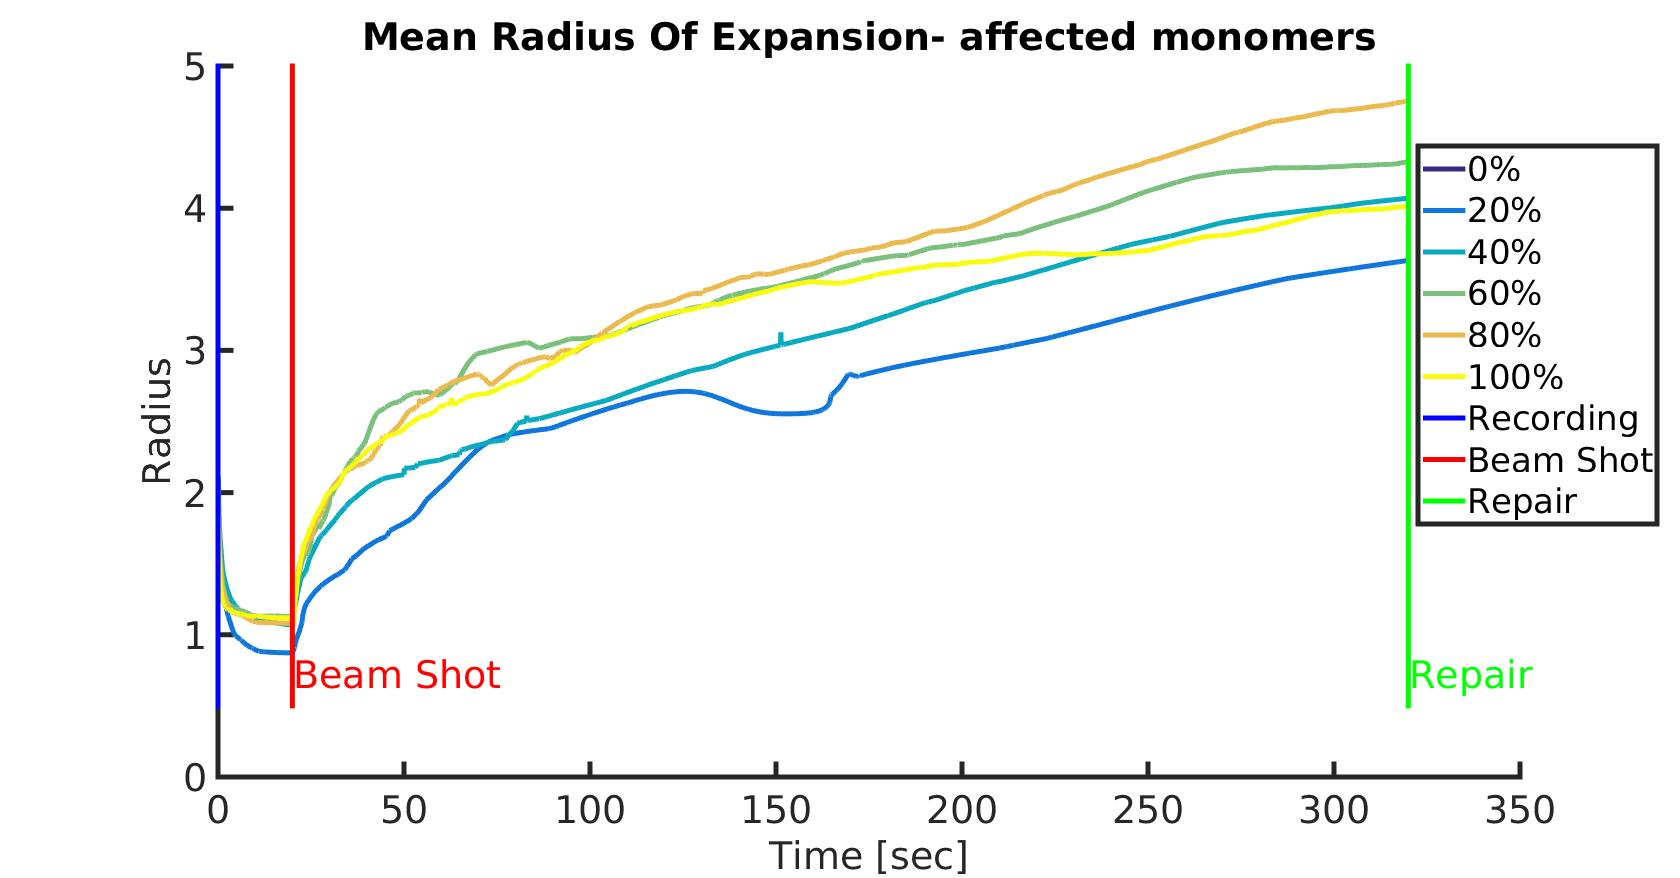
\includegraphics[width=0.5\linewidth, height=0.3\textheight]{Images/expandAffected/BreakAffectedCrosslinks/meanRadiusOfExpansionAffected}
	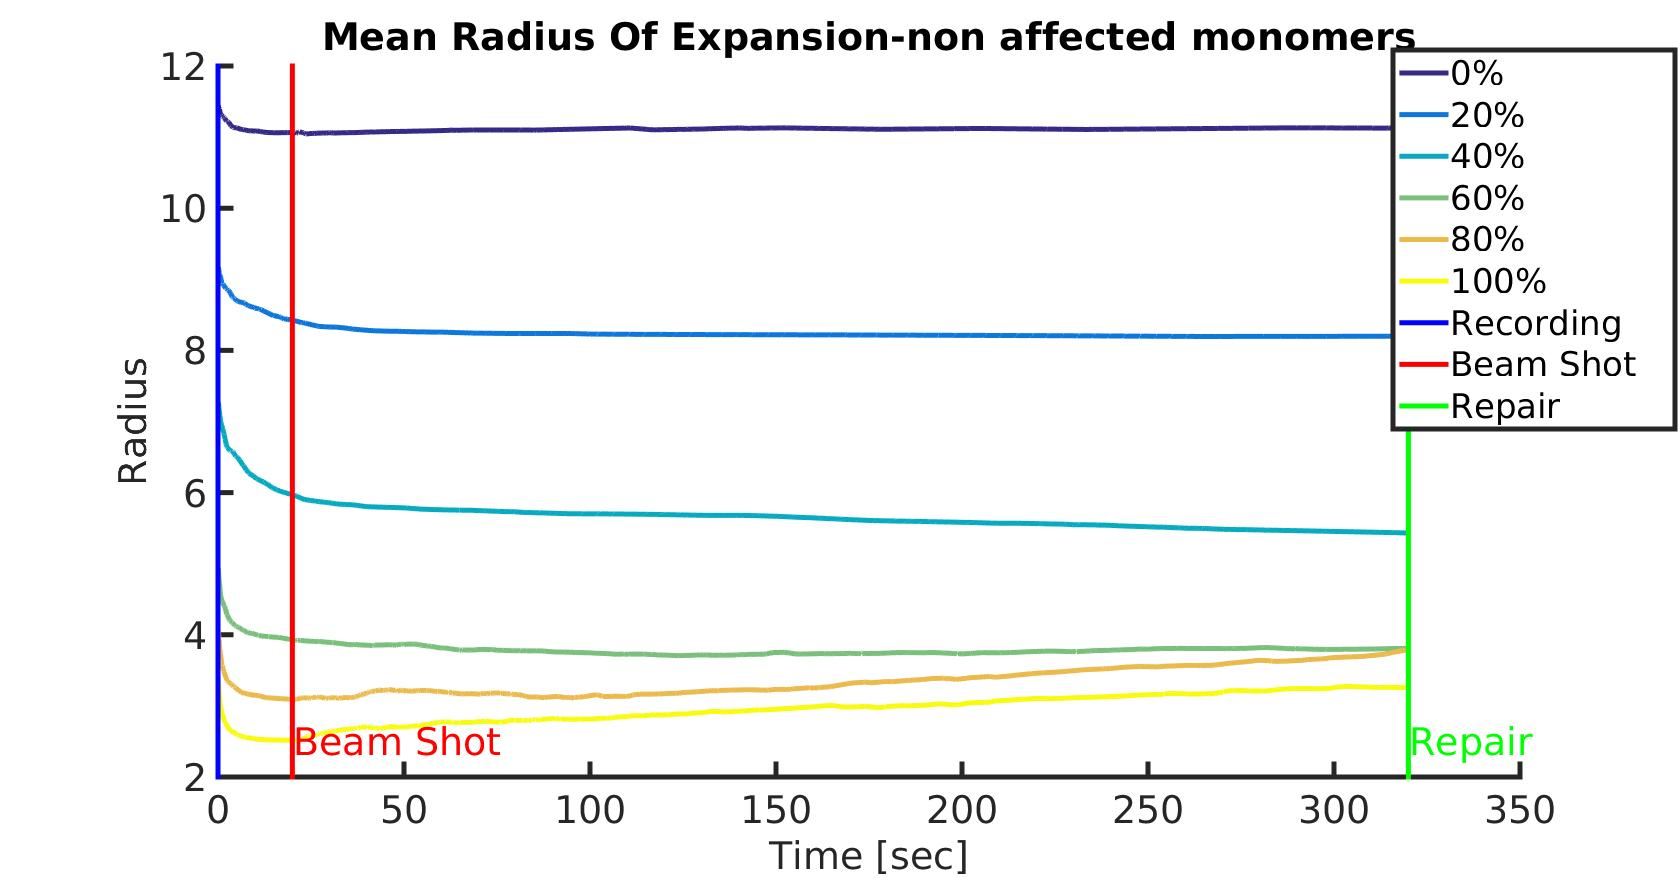
\includegraphics[width=0.5\linewidth, height=0.3\textheight]{Images/expandAffected/BreakAffectedCrosslinks/meanRadiusOfExpansionNonAffected}
	\caption{\tiny{\textbf{The radius of expansion for the affected (left) and non-affected (right) for a varying degree of connectivity. The cross-links to and from the damaged monomers are broken after UVC. As can be seen the affected monomer radius of expansion is increasing throughout the simulation, whereas the non- affected monomers remain static.  The polymer includes 500 monomers.The ROi is determined according to the damaged monomers.}}}
	\label{fig:meanRadiusOfExpansionAffectedBrokenCrosslinks}
	\end{figure}
	
	Examining the number and percentage of monomers in the ROI we have:
	
	\begin{figure}
	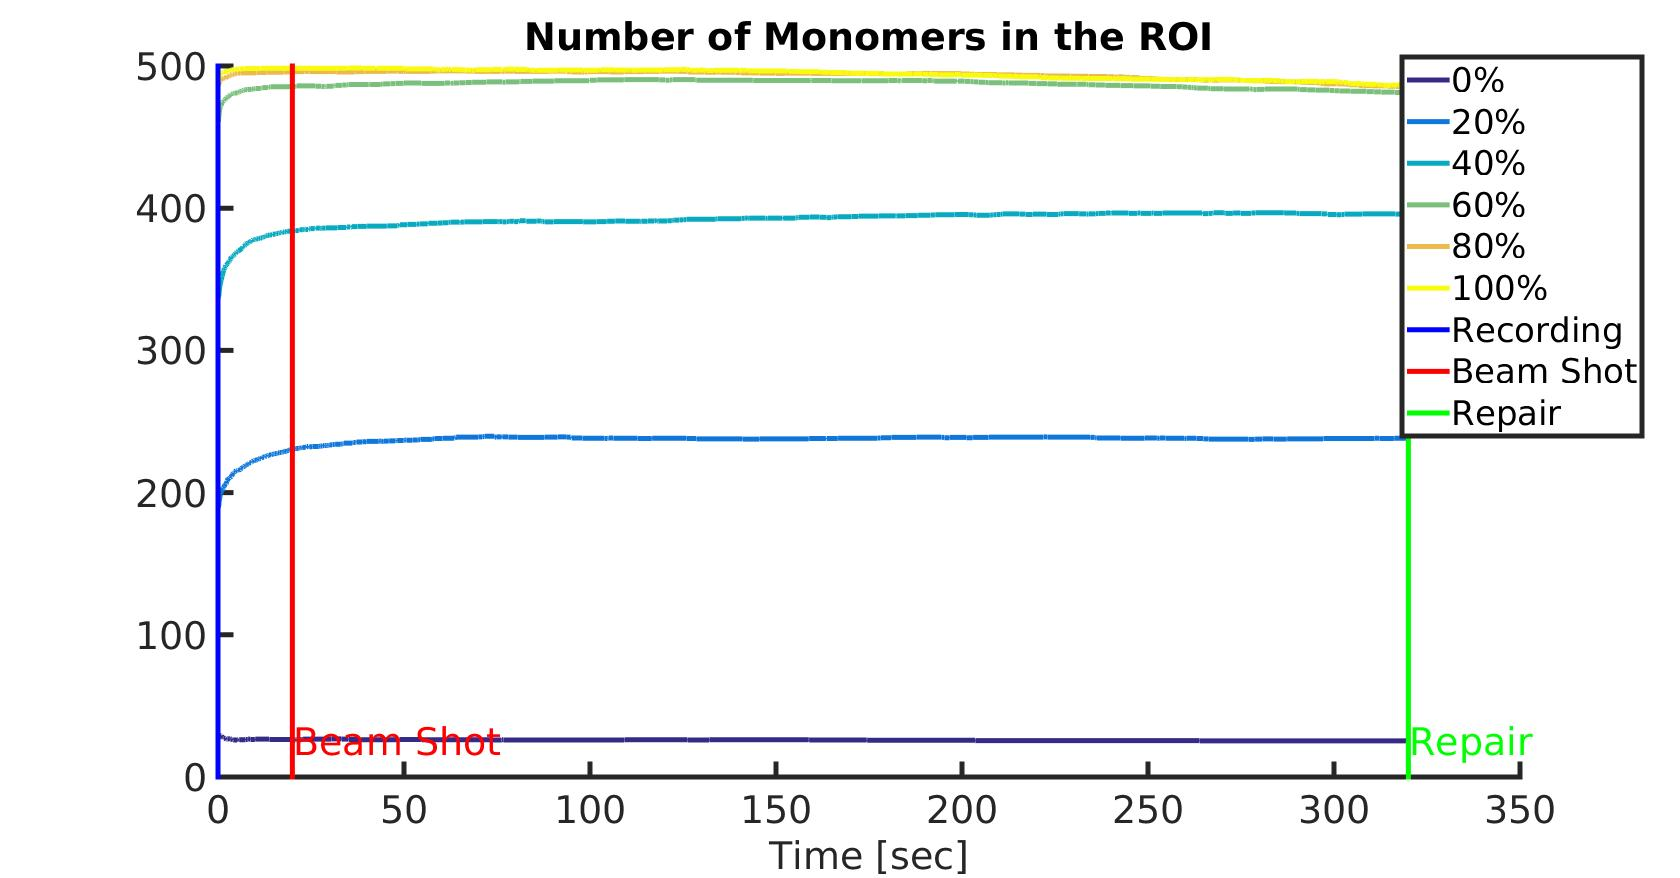
\includegraphics[width=0.5\linewidth, height=0.3\textheight]{Images/expandAffected/BreakAffectedCrosslinks/meanNumMonomersInROI}
	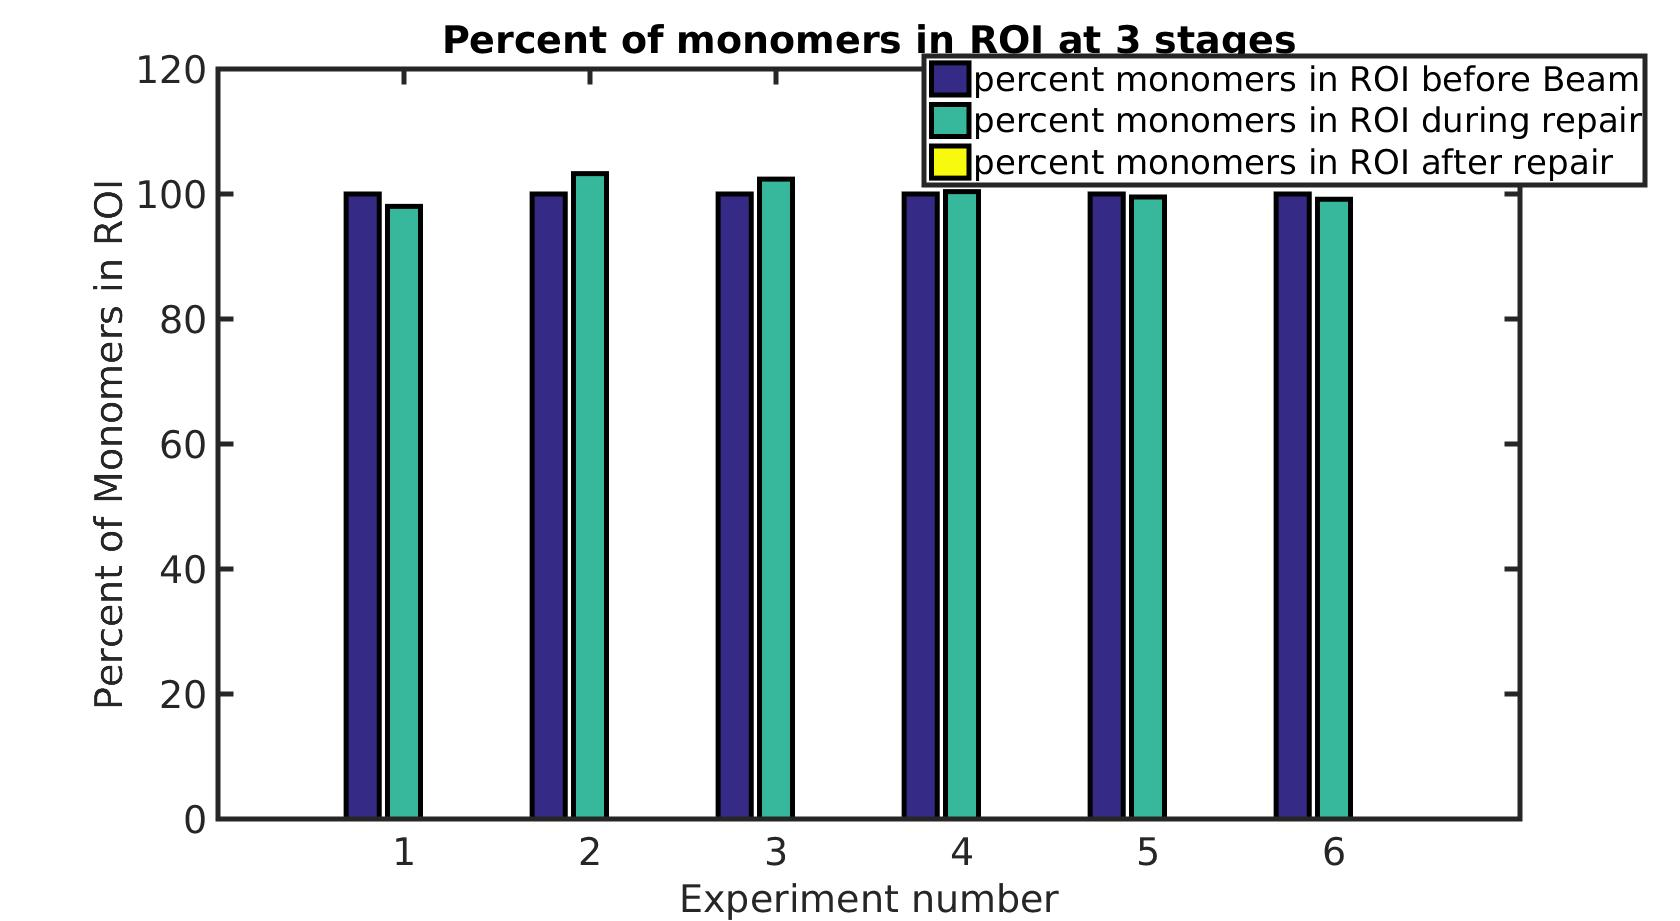
\includegraphics[width=0.5\linewidth, height=0.3\textheight]{Images/expandAffected/BreakAffectedCrosslinks/percentMonomersInROI}
	\caption{\tiny{\textbf{Number of monomers in ROI (left) and percentag (right) before and after UVC beam. No steps simulated past the repair phase. As can be seen, although the radius of the damaged monomers is increasing steadily, the number if monomers in the ROI remain roughly constant post UVC. In term of percentages, there seems to be no change.The polymer includes 500 monomers.The ROI is determined according to the damaged monomers.}}}
	\label{fig:meanNumMonomersInROI}
	\end{figure}
		
	
	\subsubsection{Keep all cross-links}
      \textbf{Experiment 1}
	   The radius of expansion of the damaged and non-damaged monomers is now examined when no cross-links are released after UVC damage. The ROI is determine according to the damaged monomers. The polymers contains 500 monomers. 
		     		     
		\begin{figure}[H]
		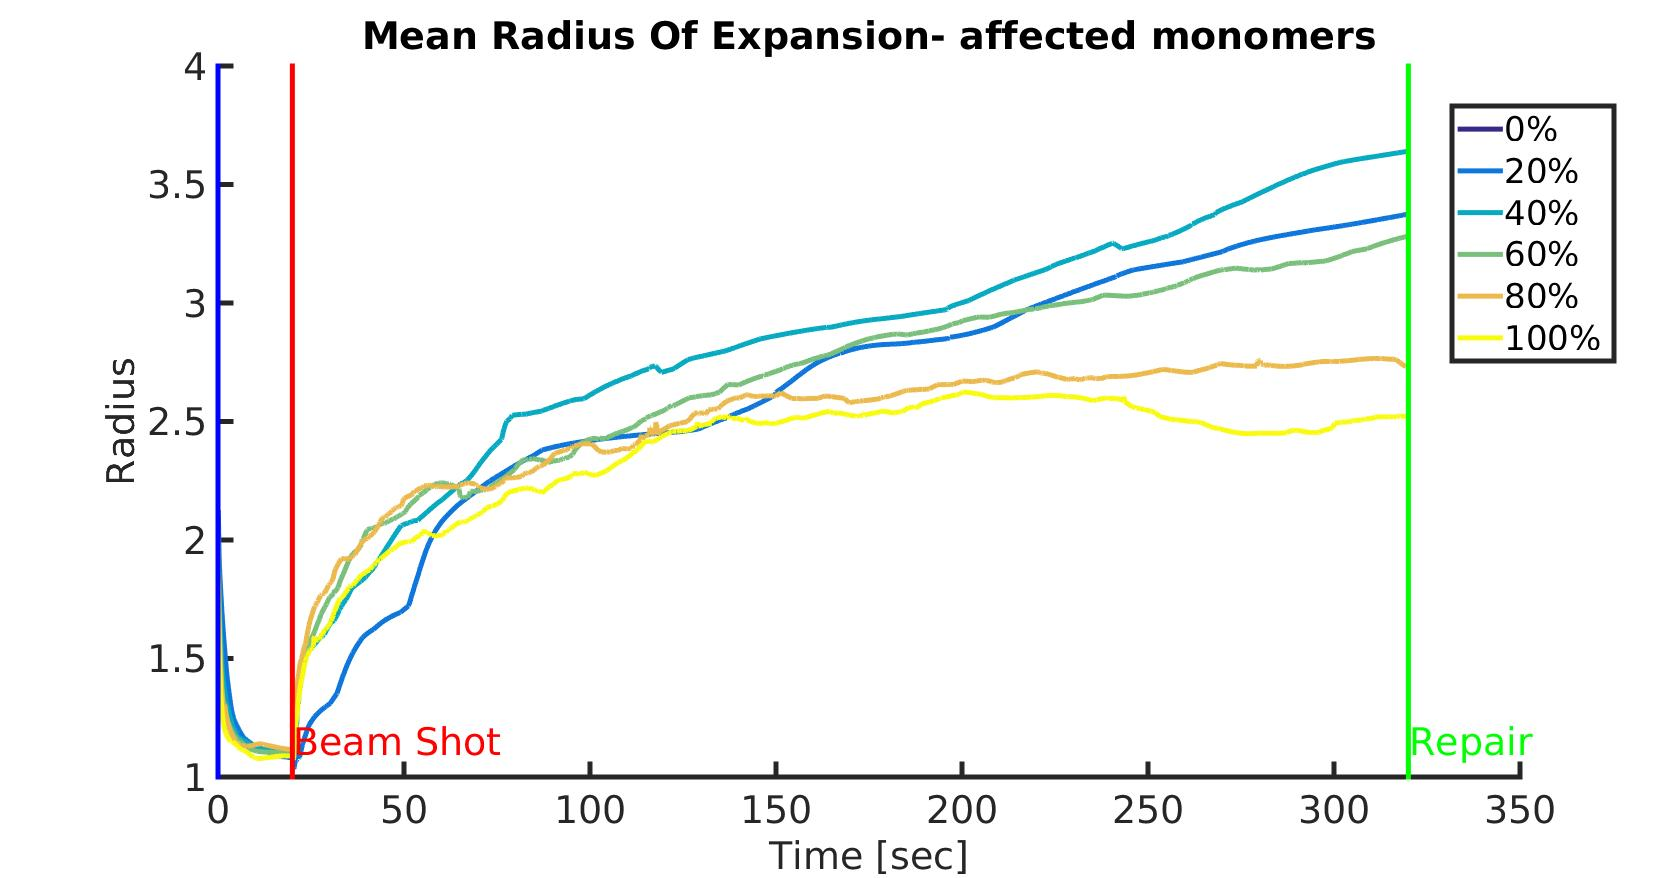
\includegraphics[width=0.5\linewidth, height=0.3\textheight]{Images/expandAffected/NoCrosslinksBroken/meanRadiusOfExpansionAffected}
		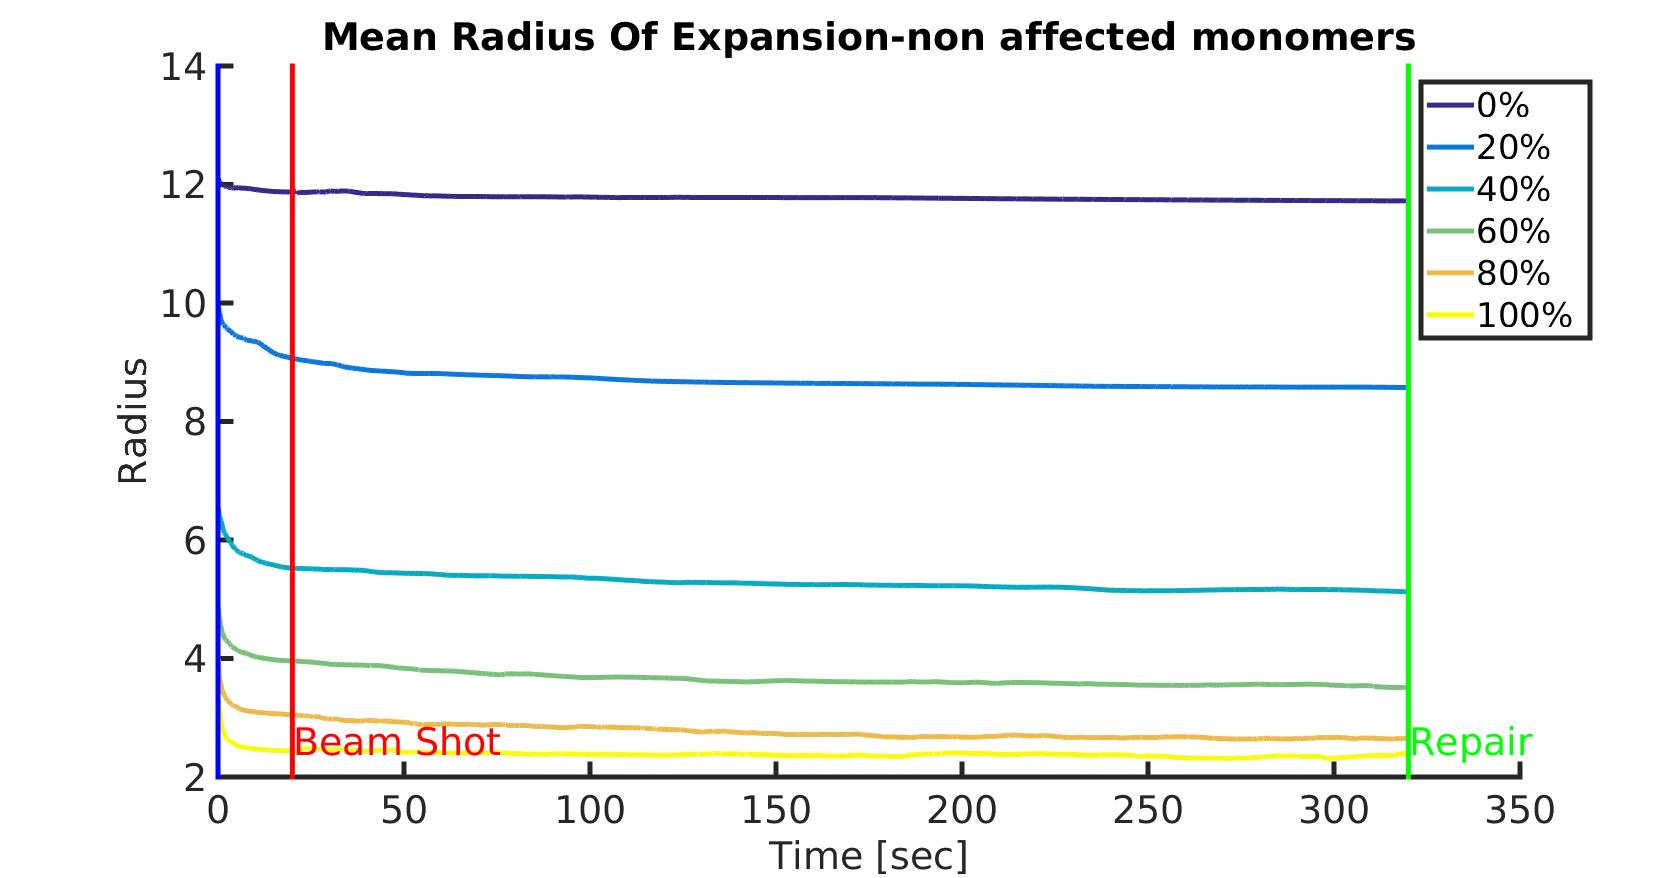
\includegraphics[width=0.5\linewidth, height=0.3\textheight]{Images/expandAffected/NoCrosslinksBroken/meanRadiusOfExpansionNonAffected}
		\caption{\tiny{\textbf{The radius of expansion for the damaged (left) and nono-damaged (right) monomers. Crosslinks are not removed after UVC. The polymer contains 500 monomers.}}}
		\label{fig:meanRadiusOfExpansionAffectedNoCrosslinksBroken}
		\end{figure}
			      
		 Examining the number and percentage of monomers in the ROI before and after UVC, we have:
		 		      
		\begin{figure}[H]
		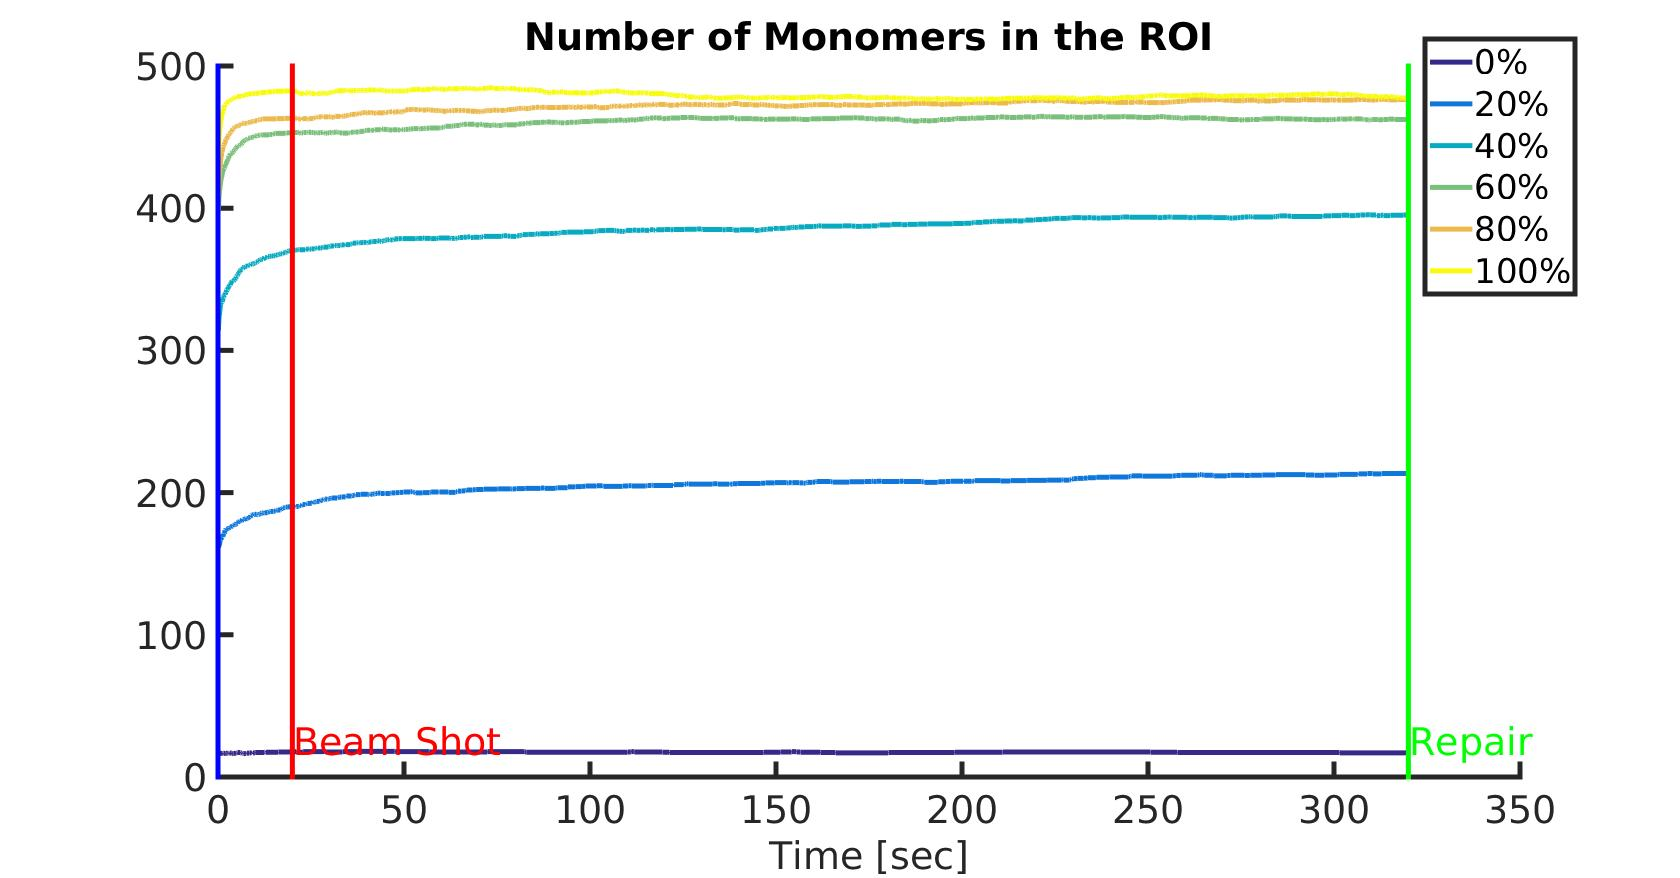
\includegraphics[width=0.5\linewidth, height=0.3\textheight]{Images/expandAffected/NoCrosslinksBroken/meanNumMonomersInROI}
		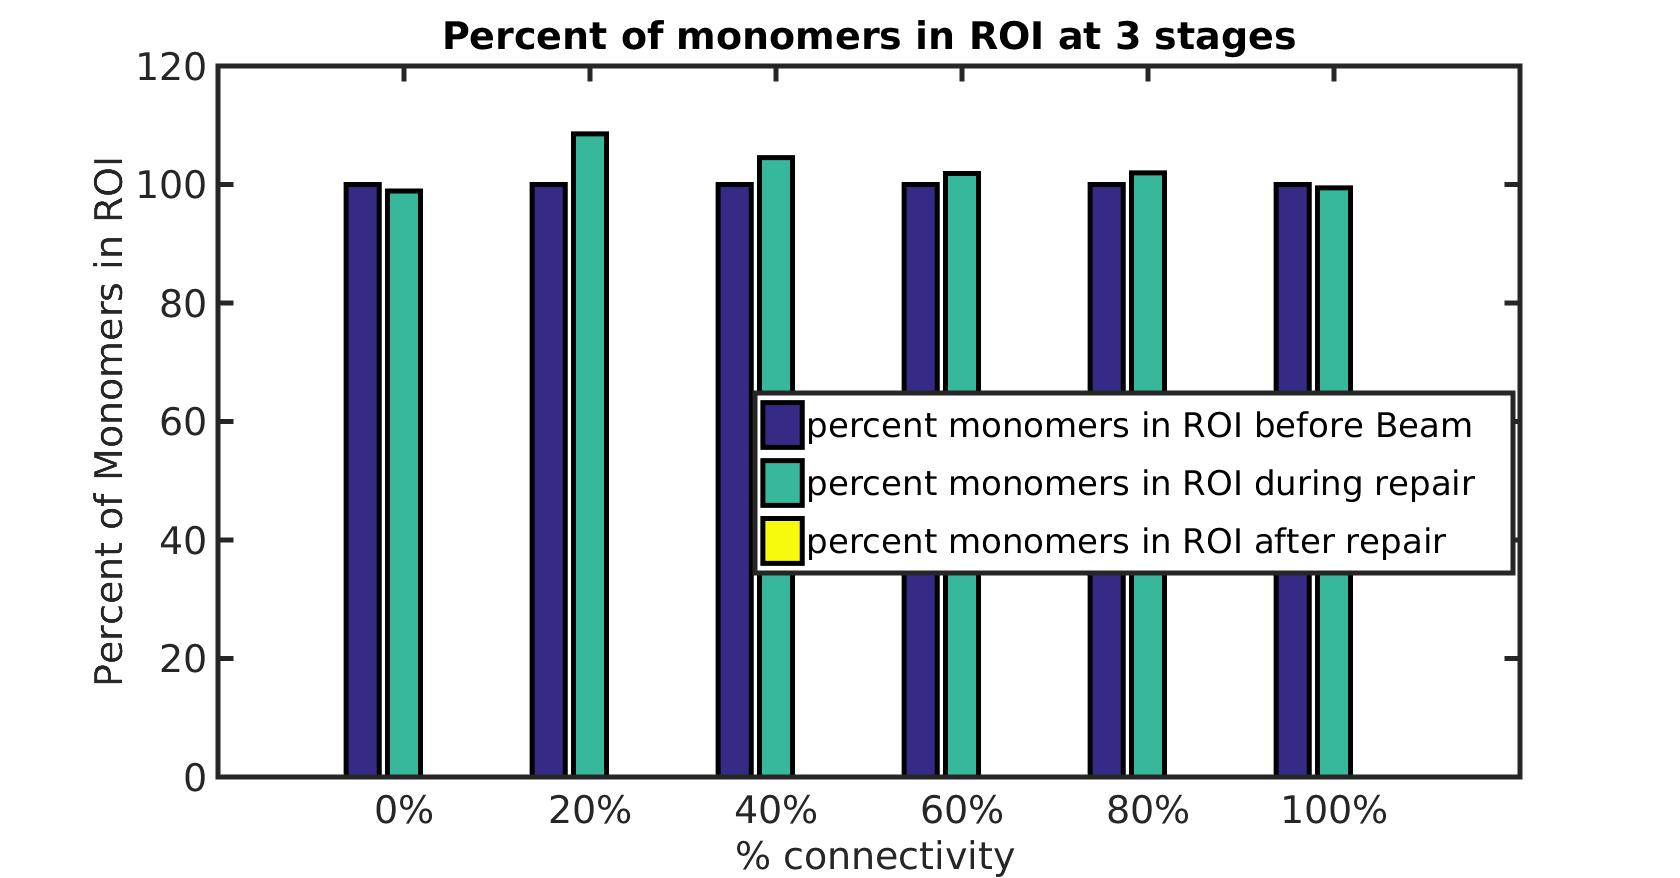
\includegraphics[width=0.5\linewidth, height=0.3\textheight]{Images/expandAffected/NoCrosslinksBroken/percentOfMonomersInROI}
		\caption{\tiny{\textbf{The number of monomers (left) and their percentages (right) in the ROI, when all crosslinks are kept after UVC. Although the radius of expansion for the affected monomers is increasing, the number of monomers in the ROI remains relatively constant. In terms of the percentages of monomers in the ROi, there seems to be no major changes. Values presented are the mean of 5 simulation with a polymer of 500 monomers for each connectivity percentage.}}}
		\label{fig:meanNumMonomersInROINoCrosslinkBroken}
		\end{figure}
		
				
	     \textbf{Experiment 2}
		     
	     We examine the radius of expansion for a more refined percentage of connectivity. when this experiment was conducted we did not yet program the ROI to be defined by the affected or non affected monomers after repair time. Therefore, the graphs of the number of monomers in the ROi and their percentages is missing. 
		     	     
	 	\begin{figure}[H]
	     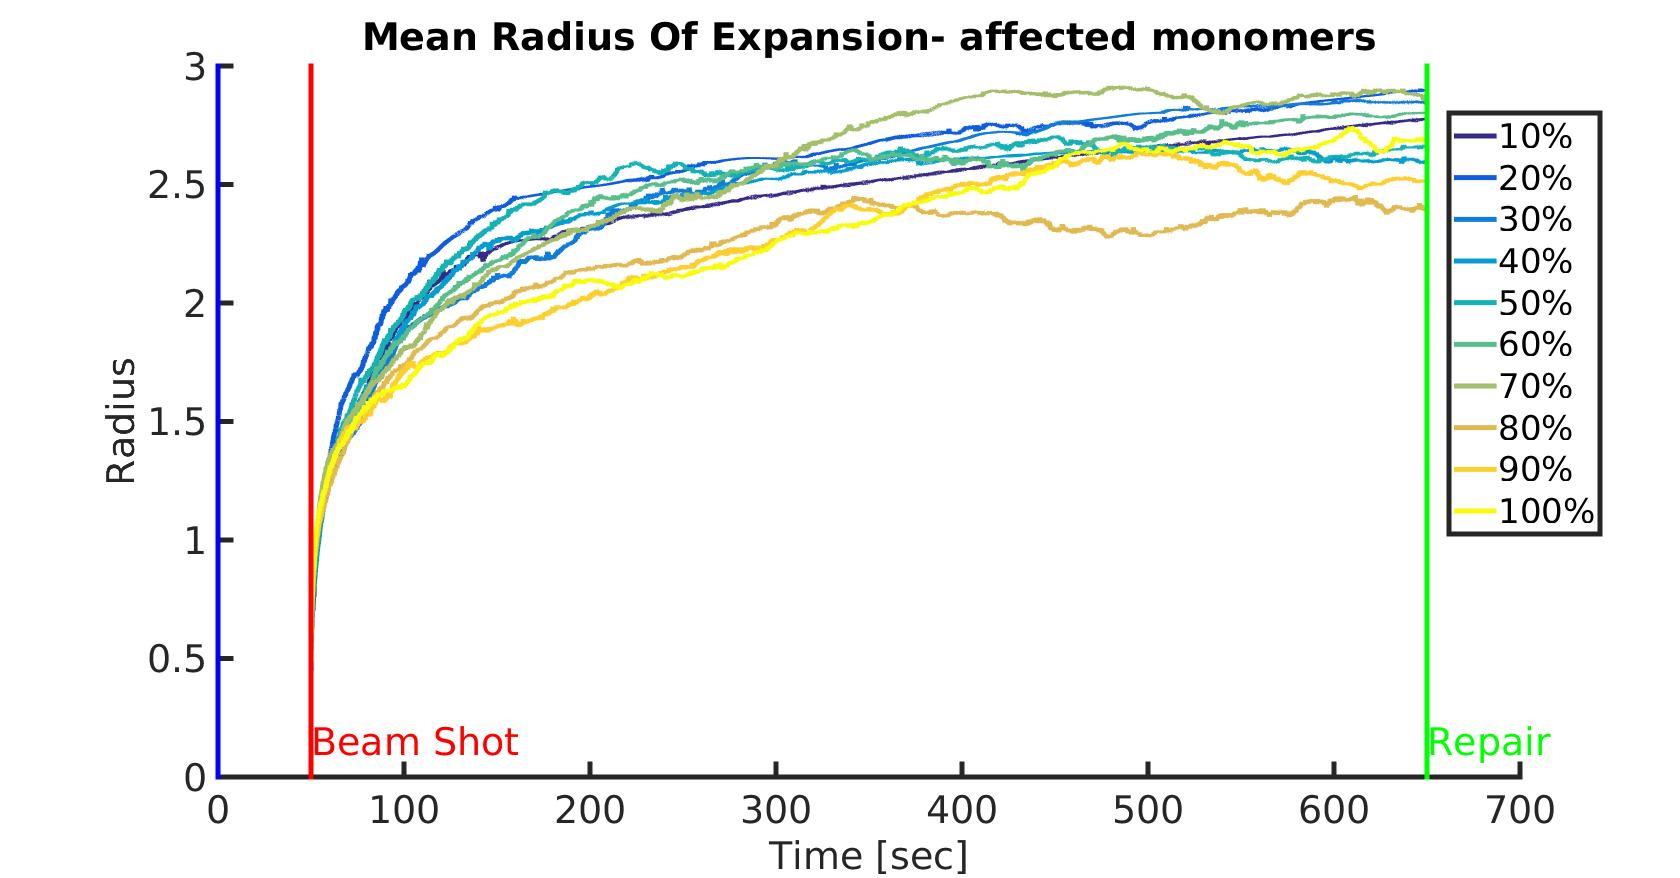
\includegraphics[width=0.5\linewidth,height=0.3\textheight]{RadiusOfExpansion500BeadsAffectedLennardJonesCrosslinked}
	     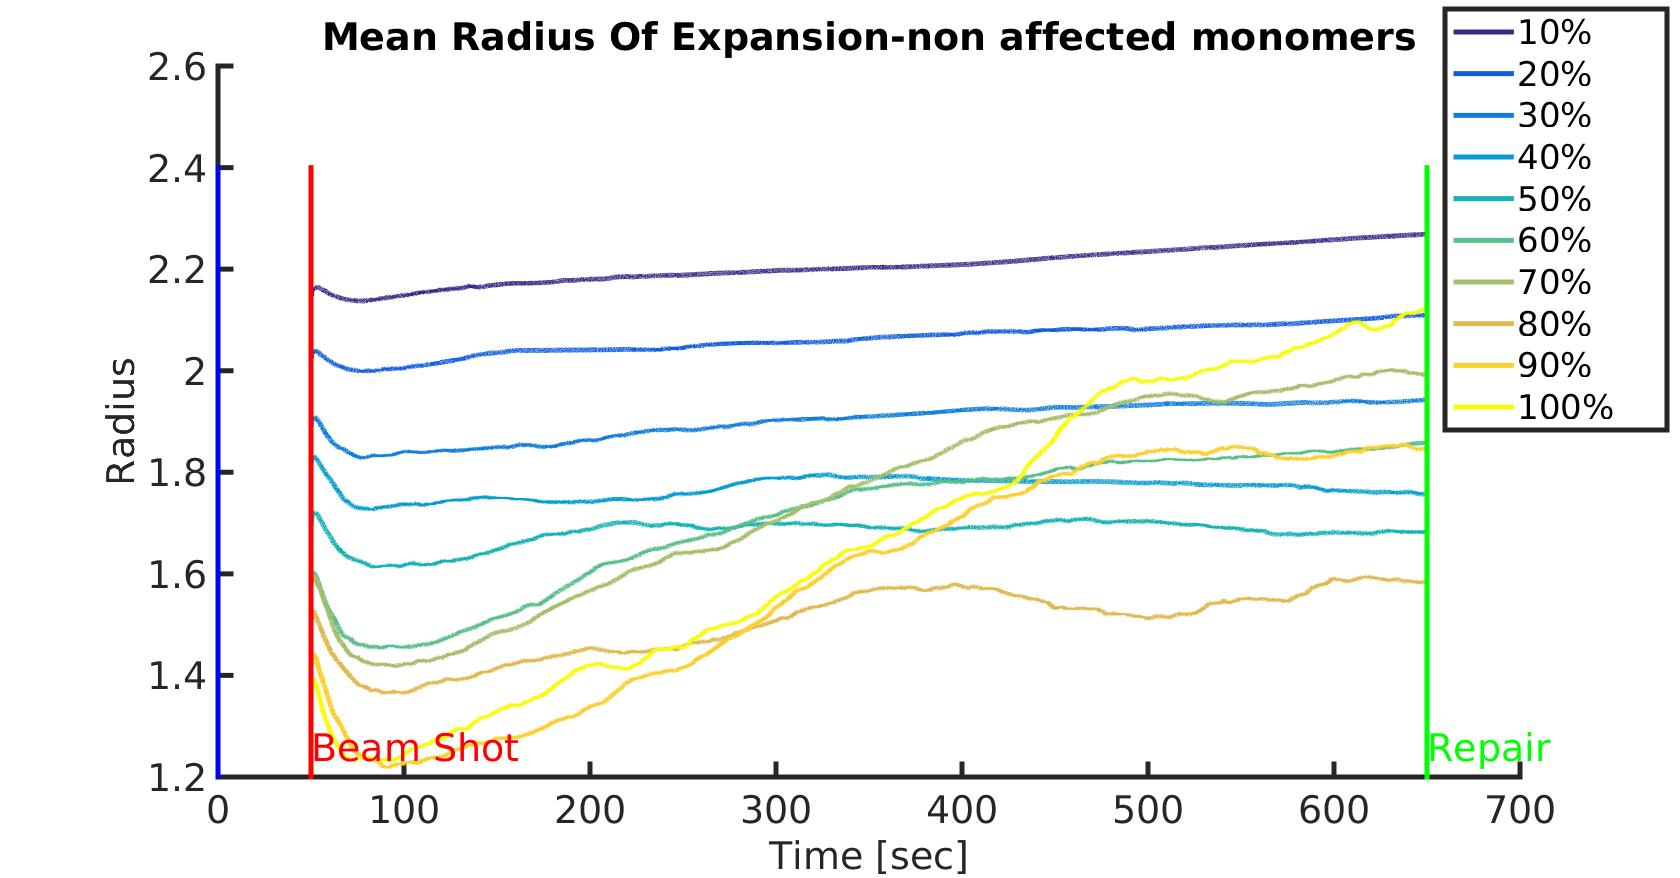
\includegraphics[width=0.5\linewidth,height=0.3\textheight]{RadiusOfExpansion500BeadsNonAffectedLennardJonesCrosslinked}
	      \caption{\tiny{\textbf{Radius of expansion for the affected (left) and non-affected (right) monomers, when the polymer is cross-linked by varying percentages. Expansion of the affected monomers is not stopped and goes beyond the non-affected expansion radius. (500 monomers with Lennard-Jones force)}}}
		     \label{fig:RadiusOfExpansion500BeadsAffectedLennardJonesCrosslinked}
    	\end{figure}
		      		
     	As can be seen from Figure \ref{fig:RadiusOfExpansion500BeadsAffectedLennardJonesCrosslinked} even with cross-links, and the given parameter set, expansion of the affected monomers is not stopped. 
	  	Because the region of interest to measure density in is determined post-prior to the expansion, this will pose a problem, since the ROI will include also the non-affected monomers, which do not seem to expand much in low percentages of cross-linking.
		      		
	  	This brings us to believe that high level of connectivity is needed, where both the affected and non-affected radius of expansion increases (see, for example, the curves for 80-100\% connectivity in Figure \ref{fig:RadiusOfExpansion500BeadsAffectedLennardJonesCrosslinked}). In that scenario, the ROI, which is determined at the end of the beam steps will more likely represent the expanded area seen in experiments, in which we see 20\% loss of material. 
		      		
	  	Two monomers of a cross-linked polymer are more likely to be found in the center. In a cross-linked polymer, after we shut-down diffusion, there is a convergence toward the center because all cross-links are pulling toward one another. This creates the situation that the affected beads do not have to expand much to pass the cross-linked layer of the non-affected monomers. 
	
	\subsection{Assign bending to non-damaged monomers}
		
		The result of the previous subsection brought us to believe that the expansion should not occur in the affected monomers but rather in the non-affected ones. The 20\% lose in DNA density should be attributed to the non-damaged monomers. The damaged DNA remains within the repair zone, whereas non-damaged DNA is pushed aside by the repair mechanism. Following this scenario, the simulation now captures the following process:
		\begin{enumerate}
			\item cross-linked polymer is being shot by UVC;
			\item cross-links to and from the damaged monomers are released;
			\item repair mechanism pushes the non-damaged monomers out of the way, this causes bending elasticity for the non-damaged monomers.
		\end{enumerate}
		
		An alternative to step 3 is to assign bending elasticity to monomers in the UVC beam but those that are undamaged. The two alternative will be examined.
		
	\subsubsection{Break damaged monomers' cross-links}
     After UVC we remove all cross-links to and from any monomer damaged. No Lennard-Jones potential is used. The ROI is determined according to the expansion of the damaged monomers, whereas we assign bending elasticity to the non-damaged monomers. 
     
     
	\begin{figure}[H]
	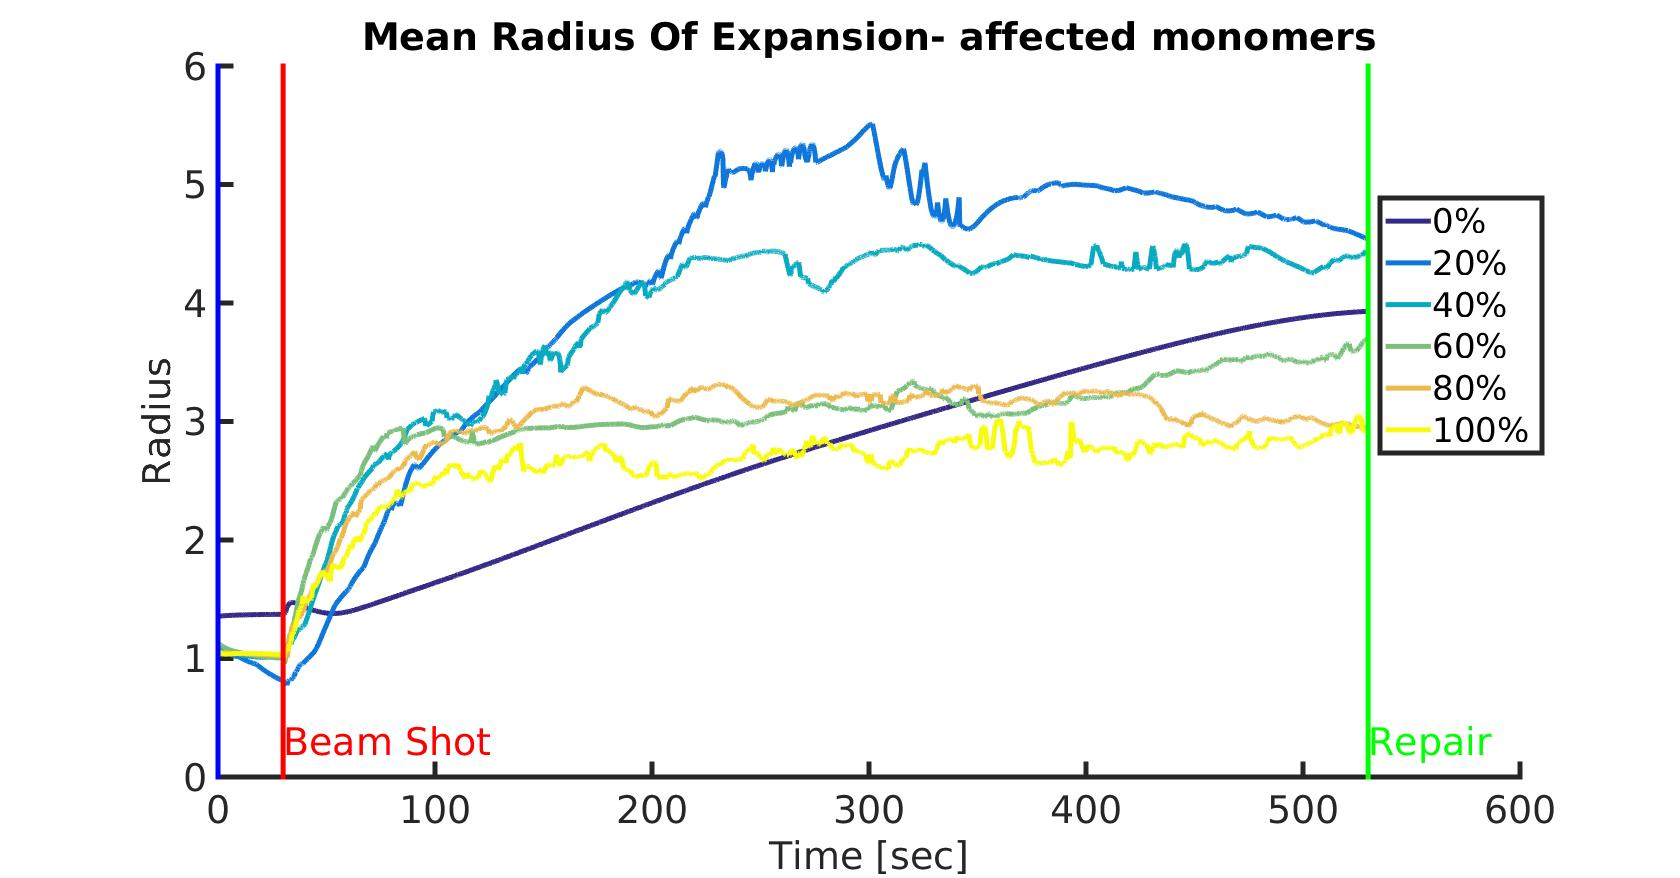
\includegraphics[width=0.5\linewidth, height=0.3\textheight]{Images/expandNonDamaged/BreakAffectedCrosslinks/04/MeanRadiusOfExpansionAffected}
    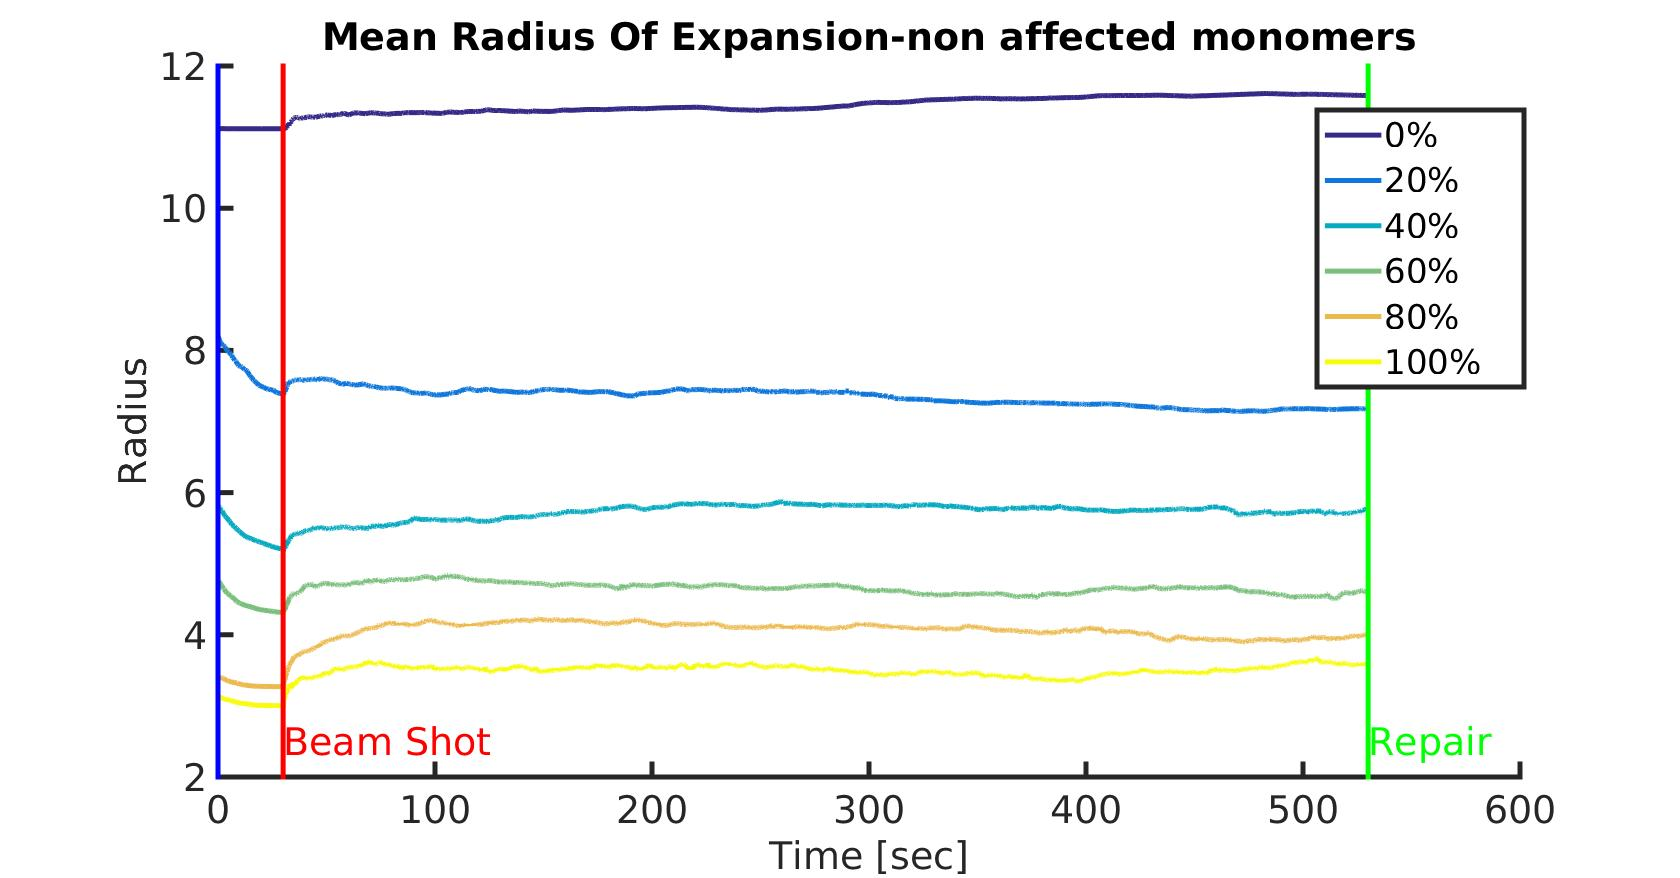
\includegraphics[width=0.5\linewidth, height=0.3\textheight]{Images/expandNonDamaged/BreakAffectedCrosslinks/04/MeanRadiusOfExpansionNonAffected}
	\caption{\tiny{\textbf{Mean Radius of expansion of the damaged (left) and non-damaged (right) monomers. As can be seen,  the radius of expansion for the affected monomers remains relatively small in comparison to the non-damaged in all experiments. (500 monomers, bending non-affected, no Lennard-Jones)}}}
	\label{fig:MeanRadiusOfExpansionAffected}
	\end{figure}
	     
	In terms of the number and percentage of monomers lose from ROI, we have:
	\begin{figure}[H]
	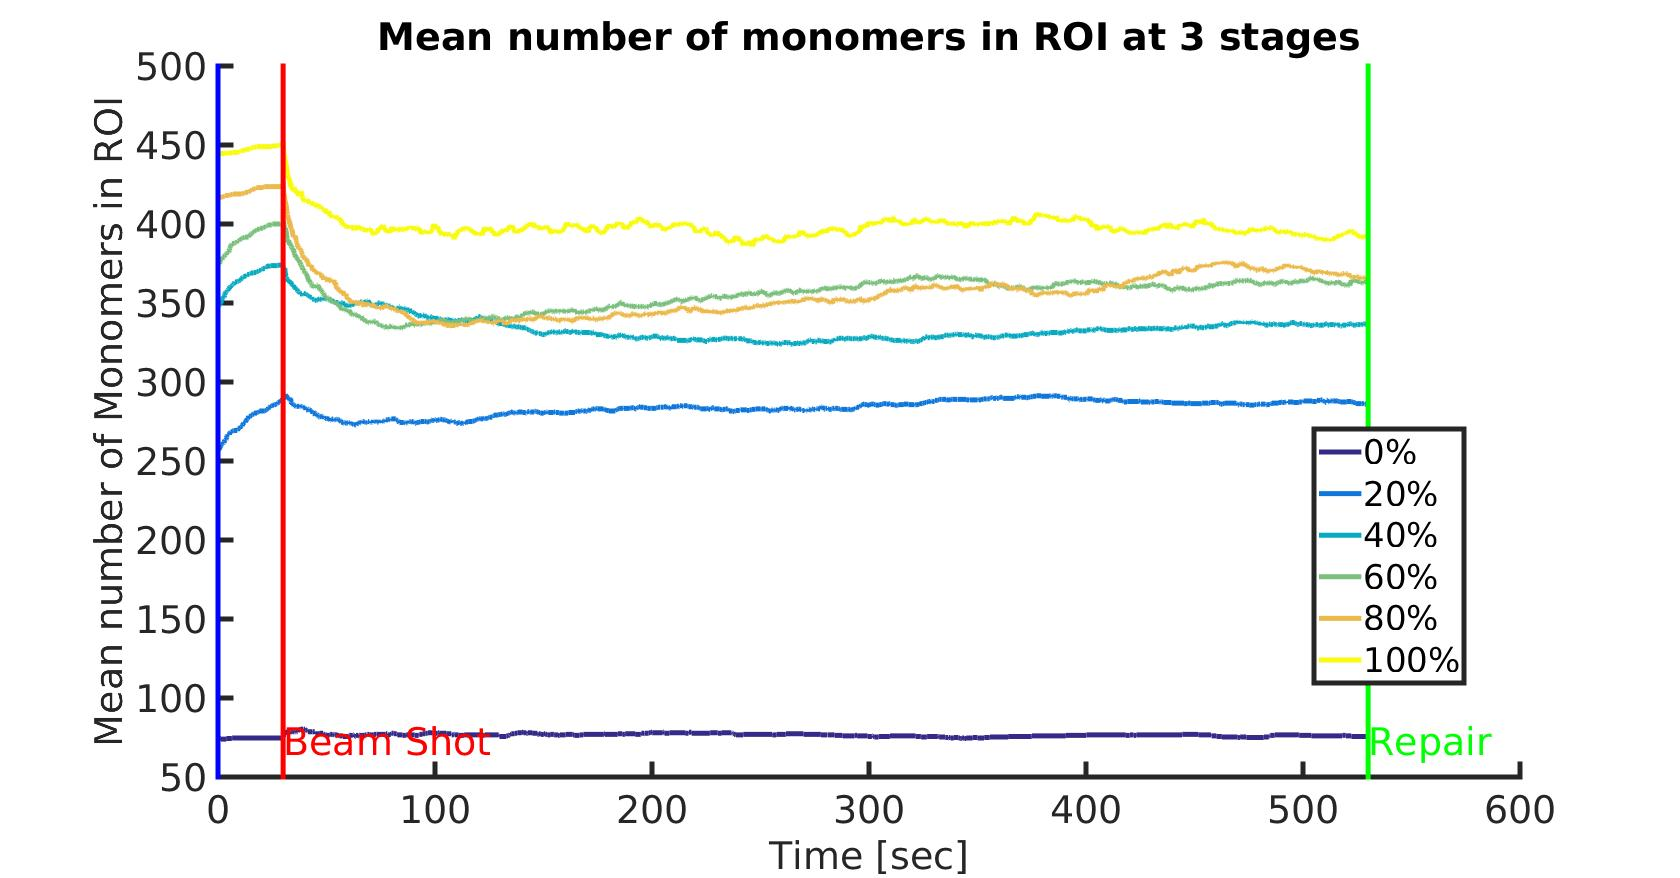
\includegraphics[width=0.5\linewidth, height=0.3\textheight]{Images/expandNonDamaged/BreakAffectedCrosslinks/04/MeanNumMonomersInROI}
	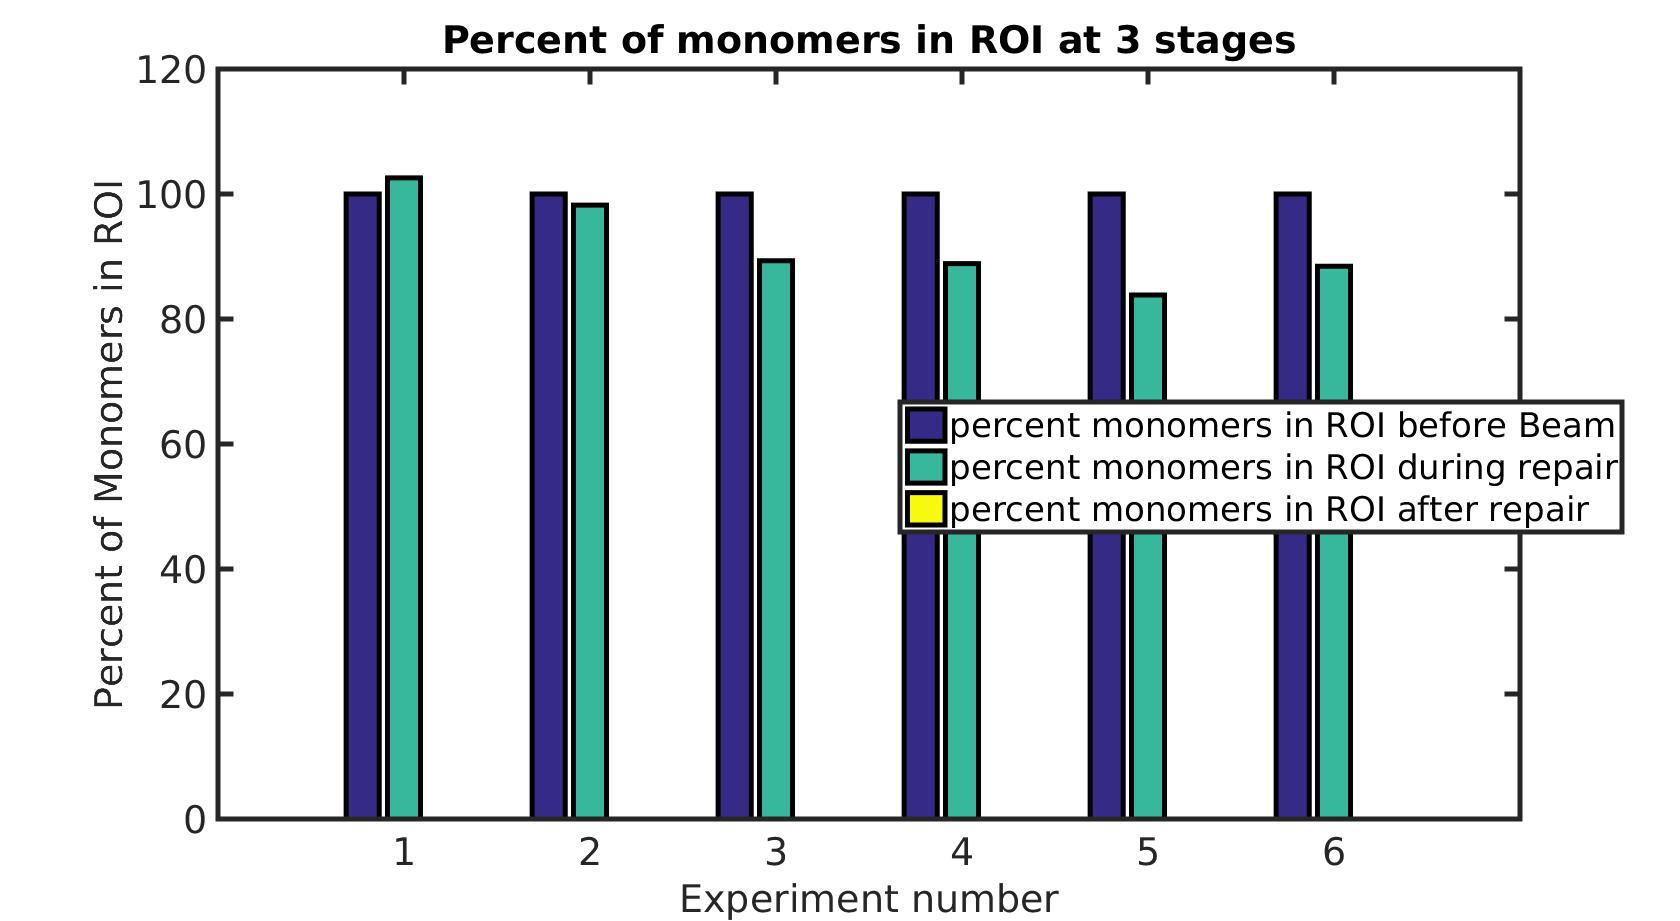
\includegraphics[width=0.5\linewidth, height=0.3\textheight]{Images/expandNonDamaged/BreakAffectedCrosslinks/04/percentOfMonomersInROI}
	\caption{\tiny{\textbf{The number of monomers in the ROI (left) with time and the overall percentage in comparison to the Recordign phase. As can be seen a loos of 20\% monomers from the ROI can be obtained with 80-100\% connectivity  (500 monomers, expanding non-affected, non Lennard-Jones)}}}
	\label{fig:MeanNumMonomersInROI}
	\end{figure}
	     For 80-100\% connectivity we can gain loss of 20\% monomers from the ROI. We now turn to explore more in-depth the parameters around 80\% connectivity. 
	     										
		\begin{figure}[H]
		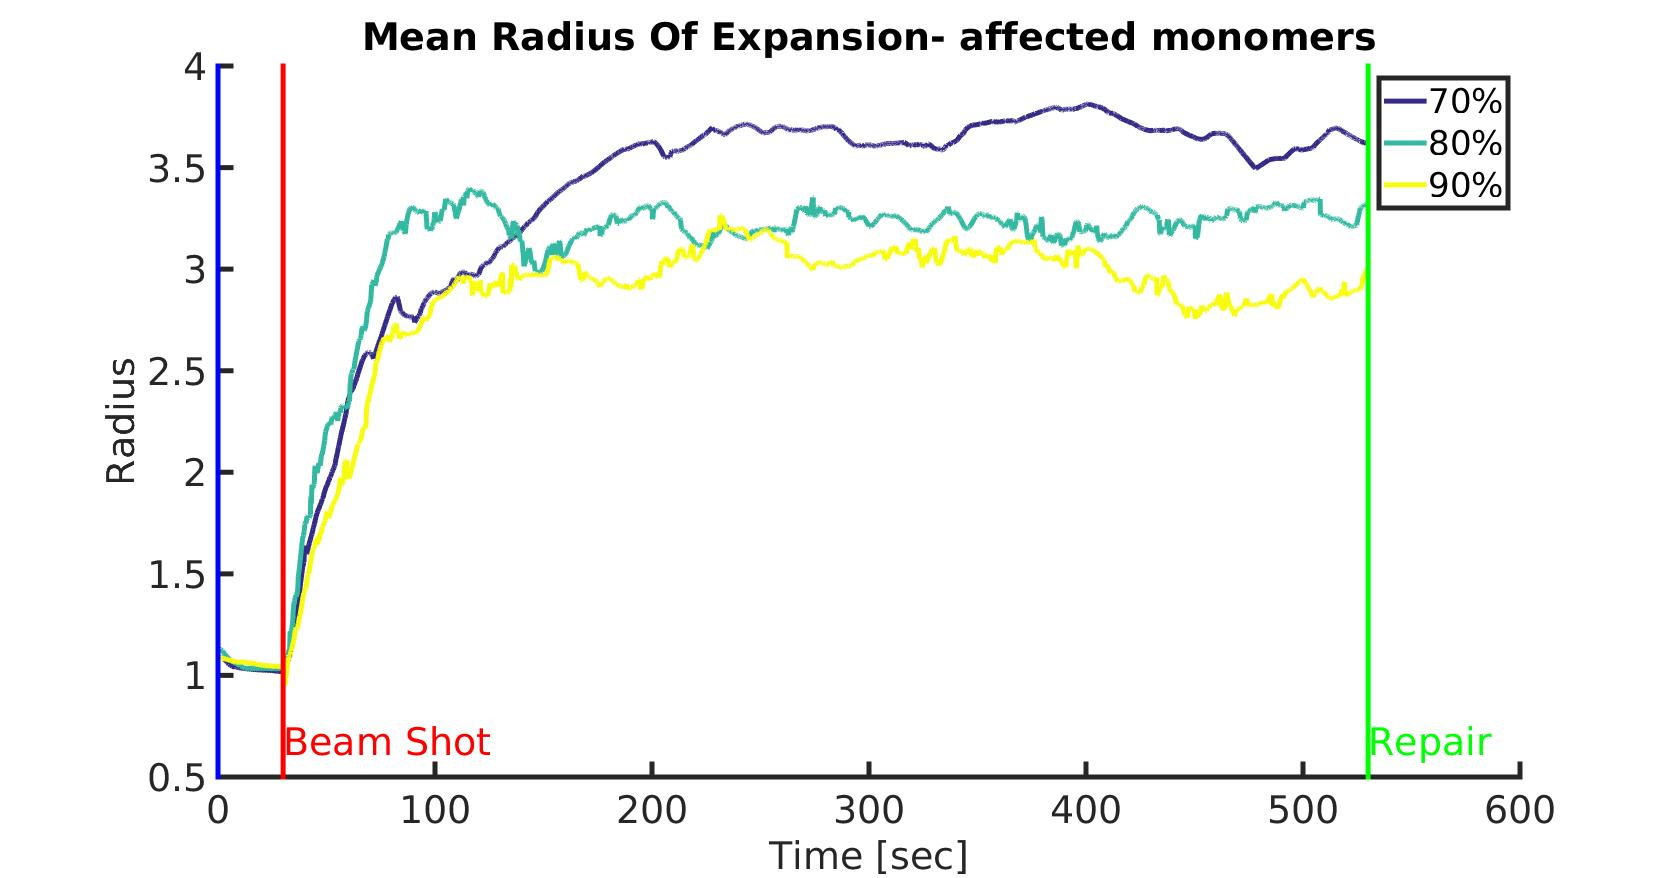
\includegraphics[width=0.5\linewidth, height=0.3\textheight]{Images/expandNonDamaged/BreakAffectedCrosslinks/05/meanRadiusOfExpansionAffected}
	    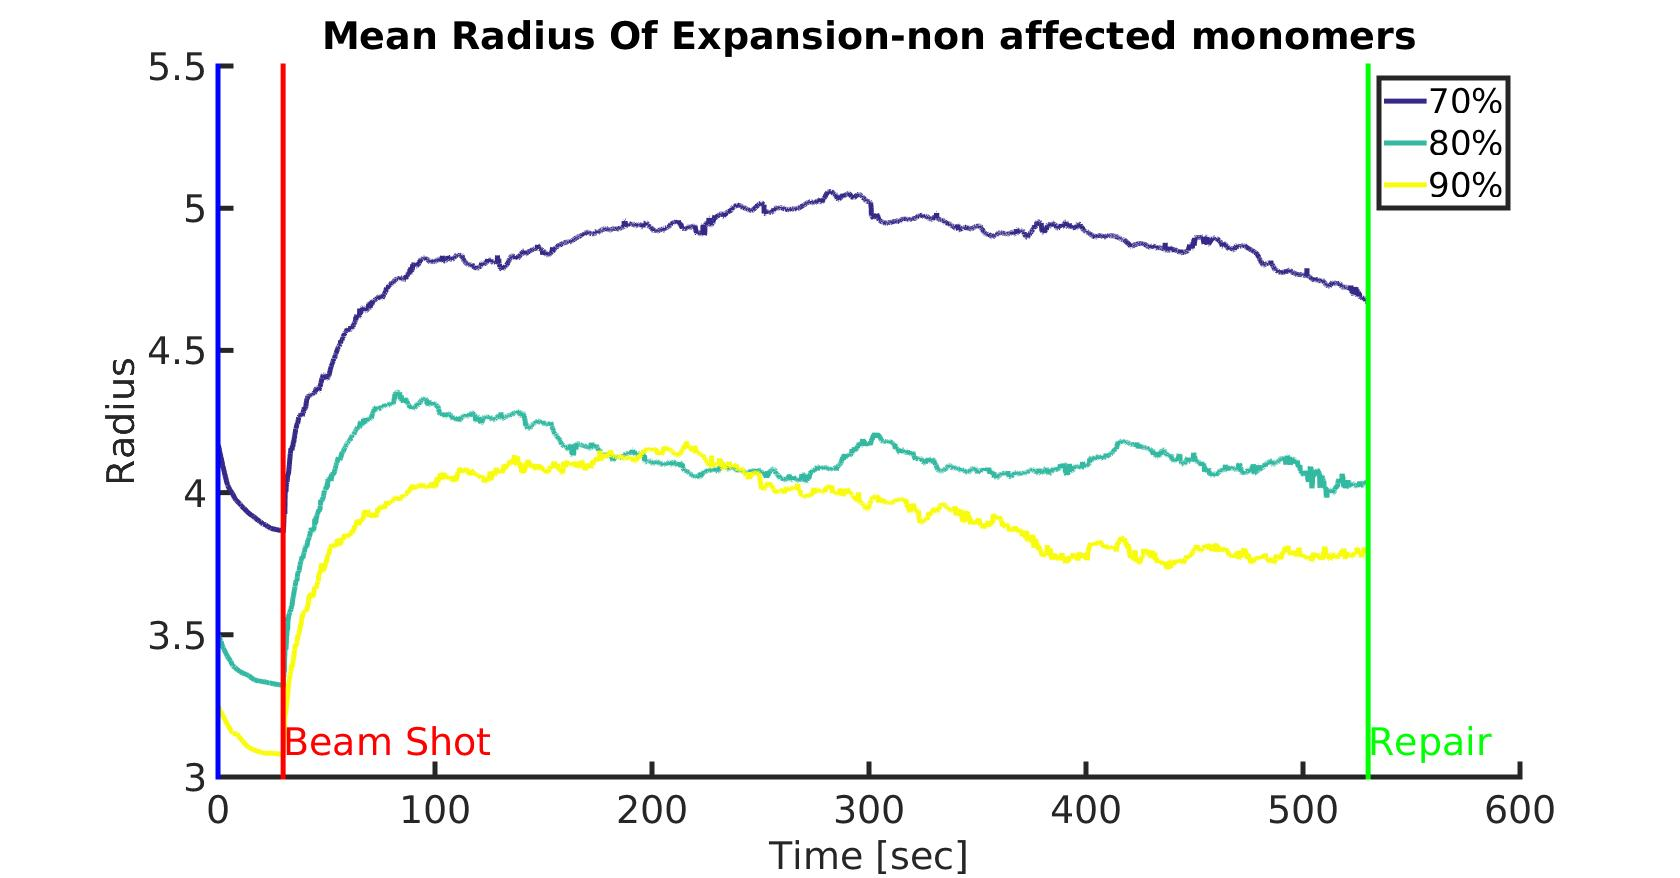
\includegraphics[width=0.5\linewidth,
		height=0.3\textheight]{Images/expandNonDamaged/BreakAffectedCrosslinks/05/meanRadiusOfExpansionNonAffected}
		\caption{}
		\label{fig:meanRadiusOfExpansionBendingNonAffectedBreakDamagedCrosslinks}
		\end{figure}
		
			
		\begin{figure}[H]
		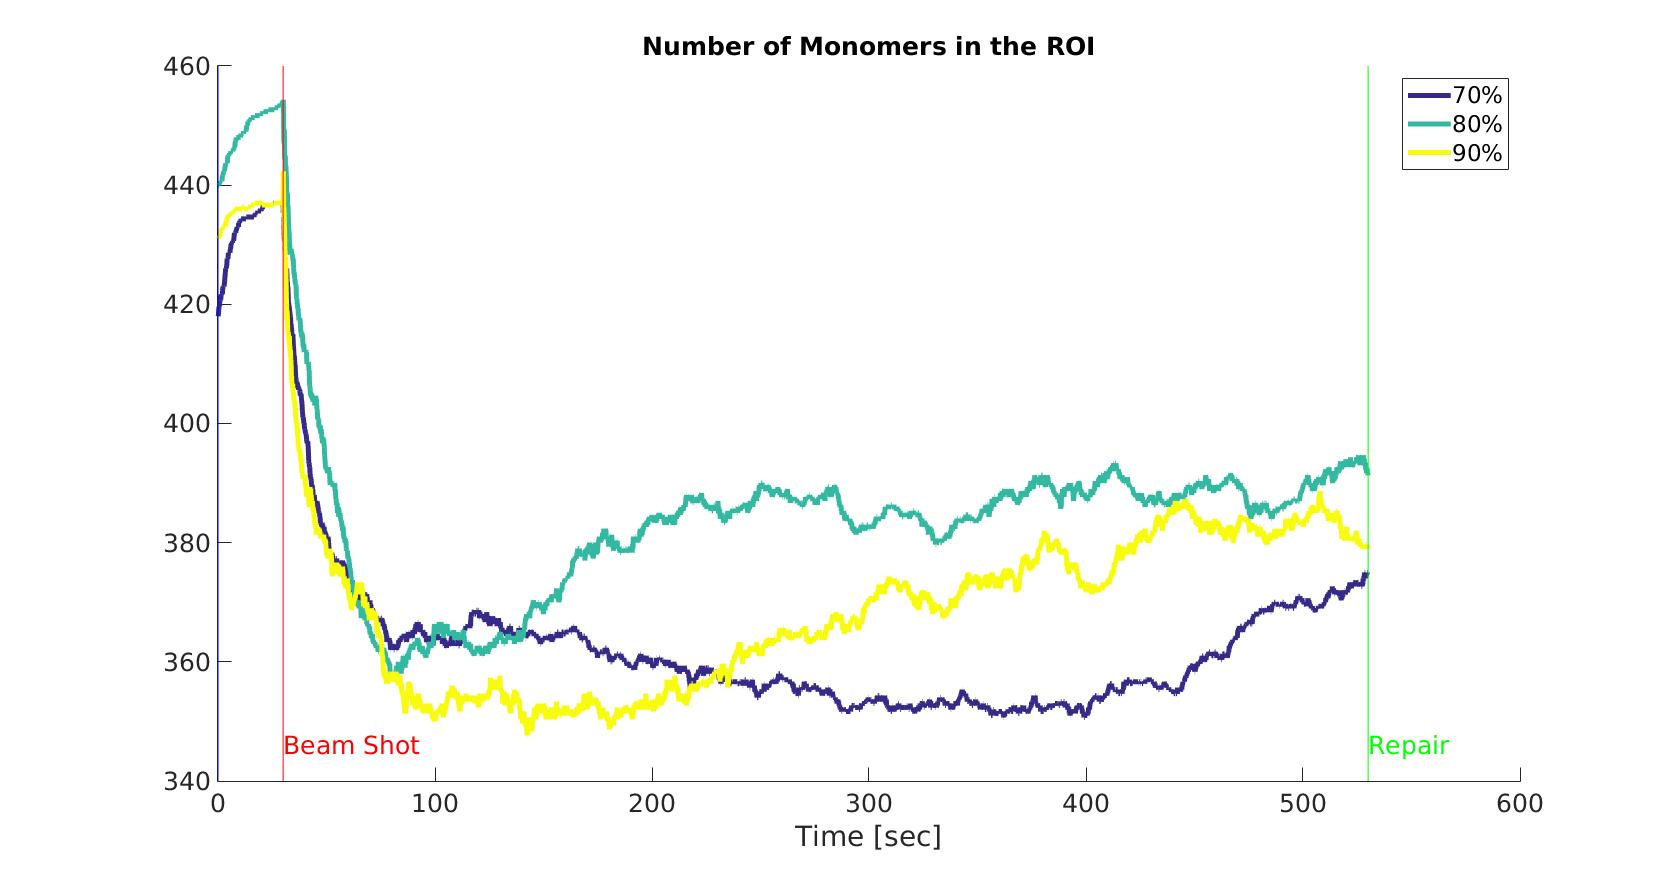
\includegraphics[width=0.5\linewidth, height=0.3\textheight]{Images/expandNonDamaged/BreakAffectedCrosslinks/05/meanNumMonomersInROI}
		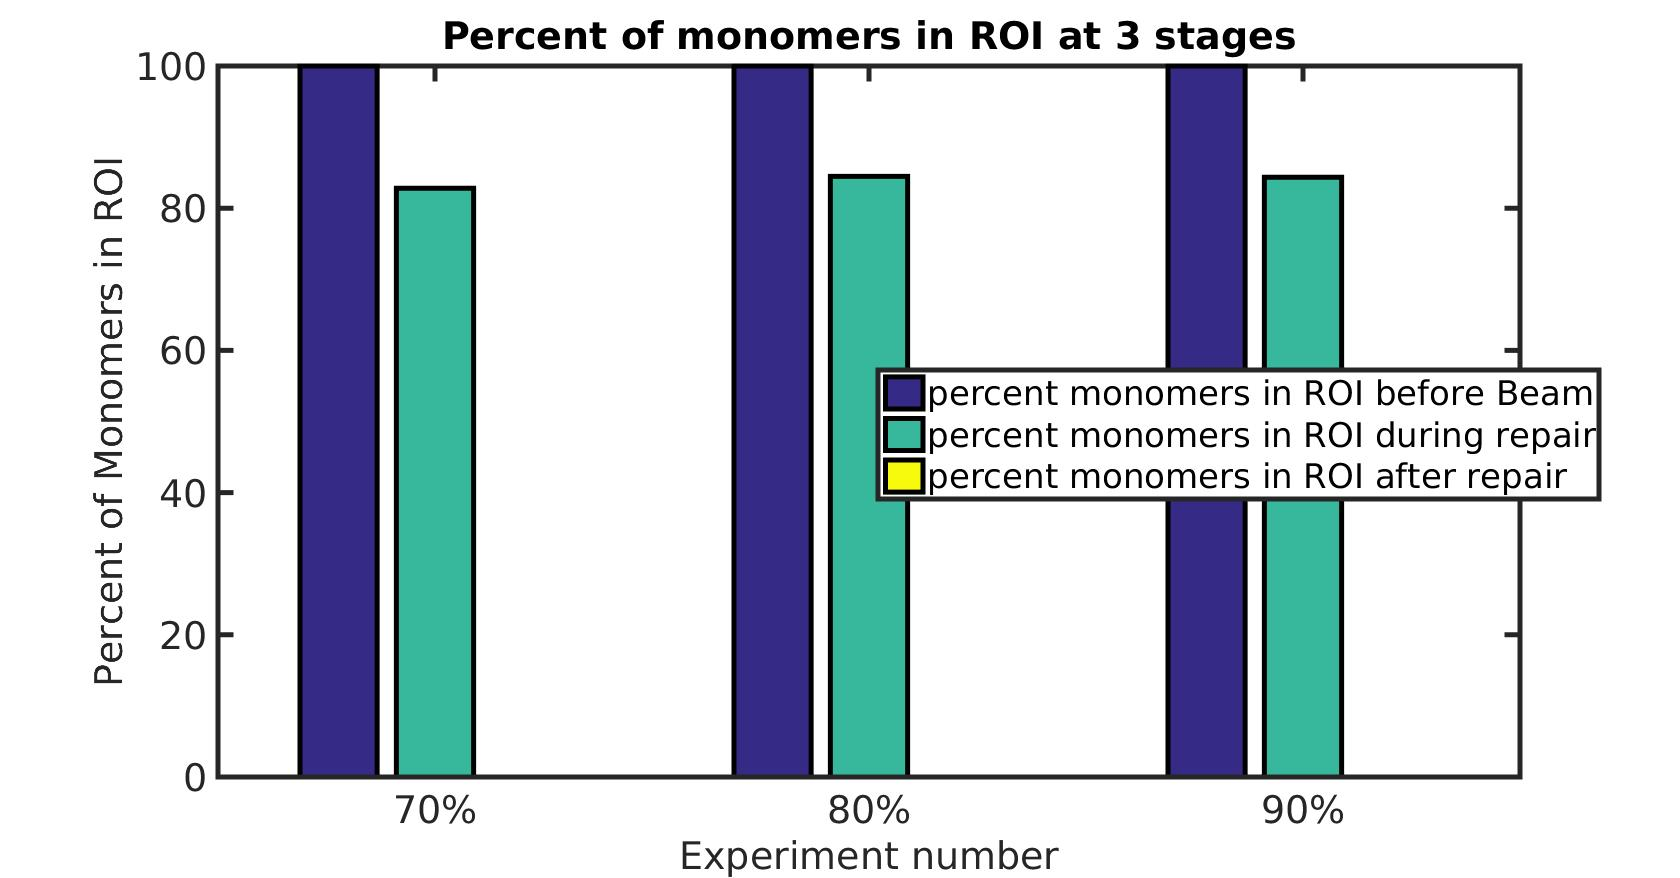
\includegraphics[width=0.5\linewidth, height=0.3\textheight]{Images/expandNonDamaged/BreakAffectedCrosslinks/05/percentageOfMonomersInROI}
		\caption{}		
		\label{fig:percentageOfMonomersInROI}
		\end{figure}
		
		
			
	\subsubsection{Keeping all cross-links after UVC}
		Keeping all cross-links, either	inside or outside the beam, while assigning bending only to non-damaged monomers we have:
		
	\begin{figure}[H]
	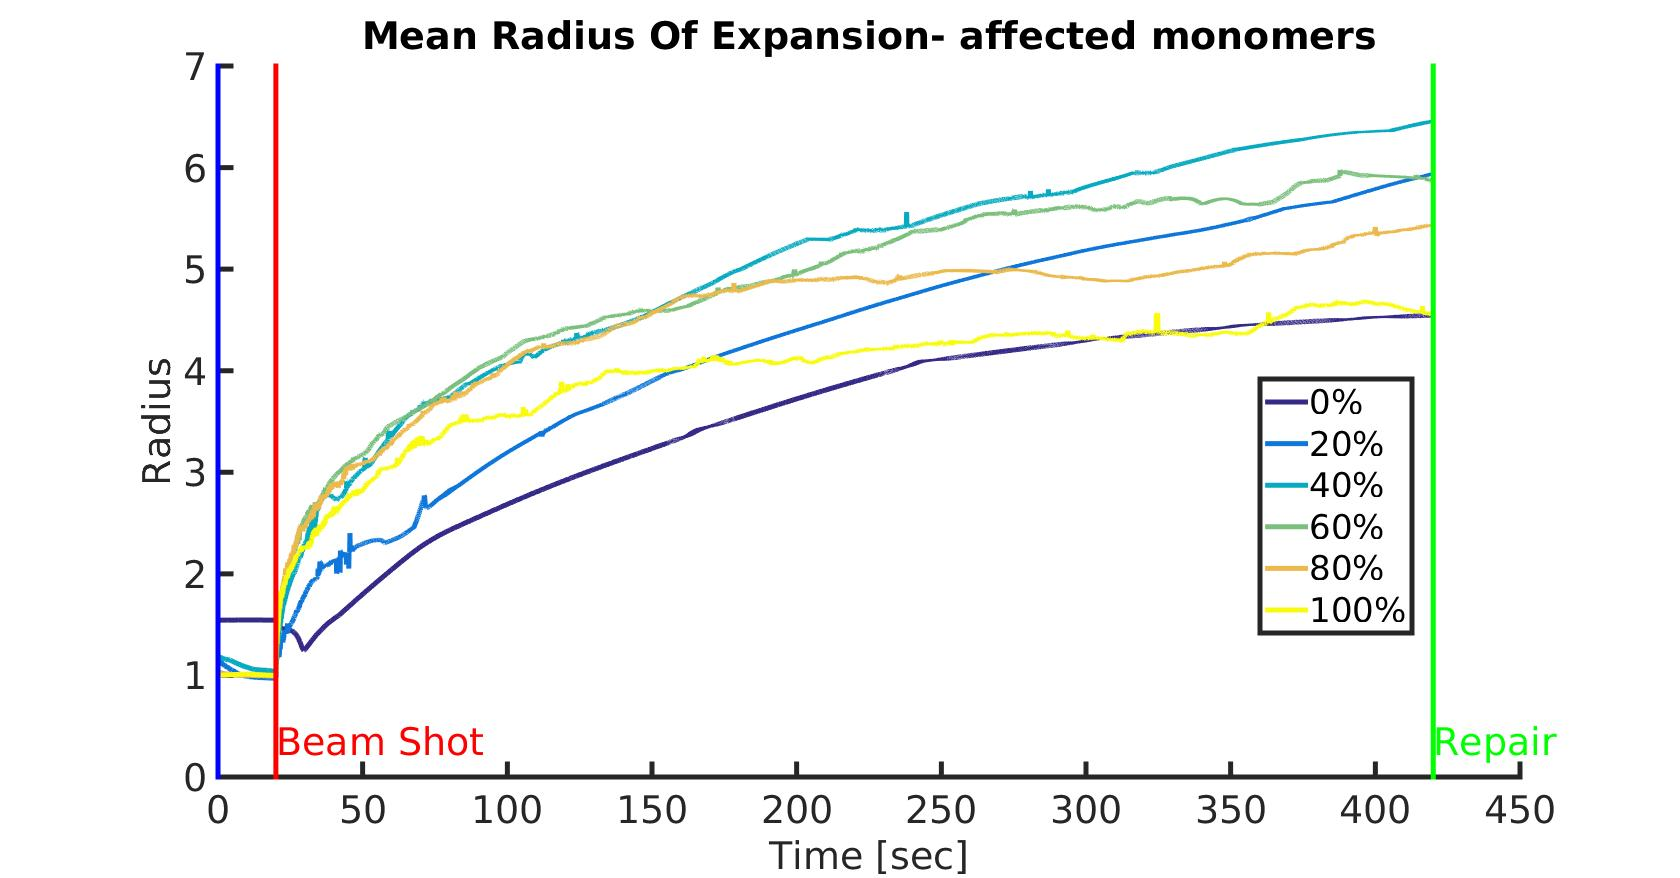
\includegraphics[width=0.5\linewidth]{Images/expandNonDamaged/NoCrosslinksBroken/meanRadiusOfExpansionAffected}
	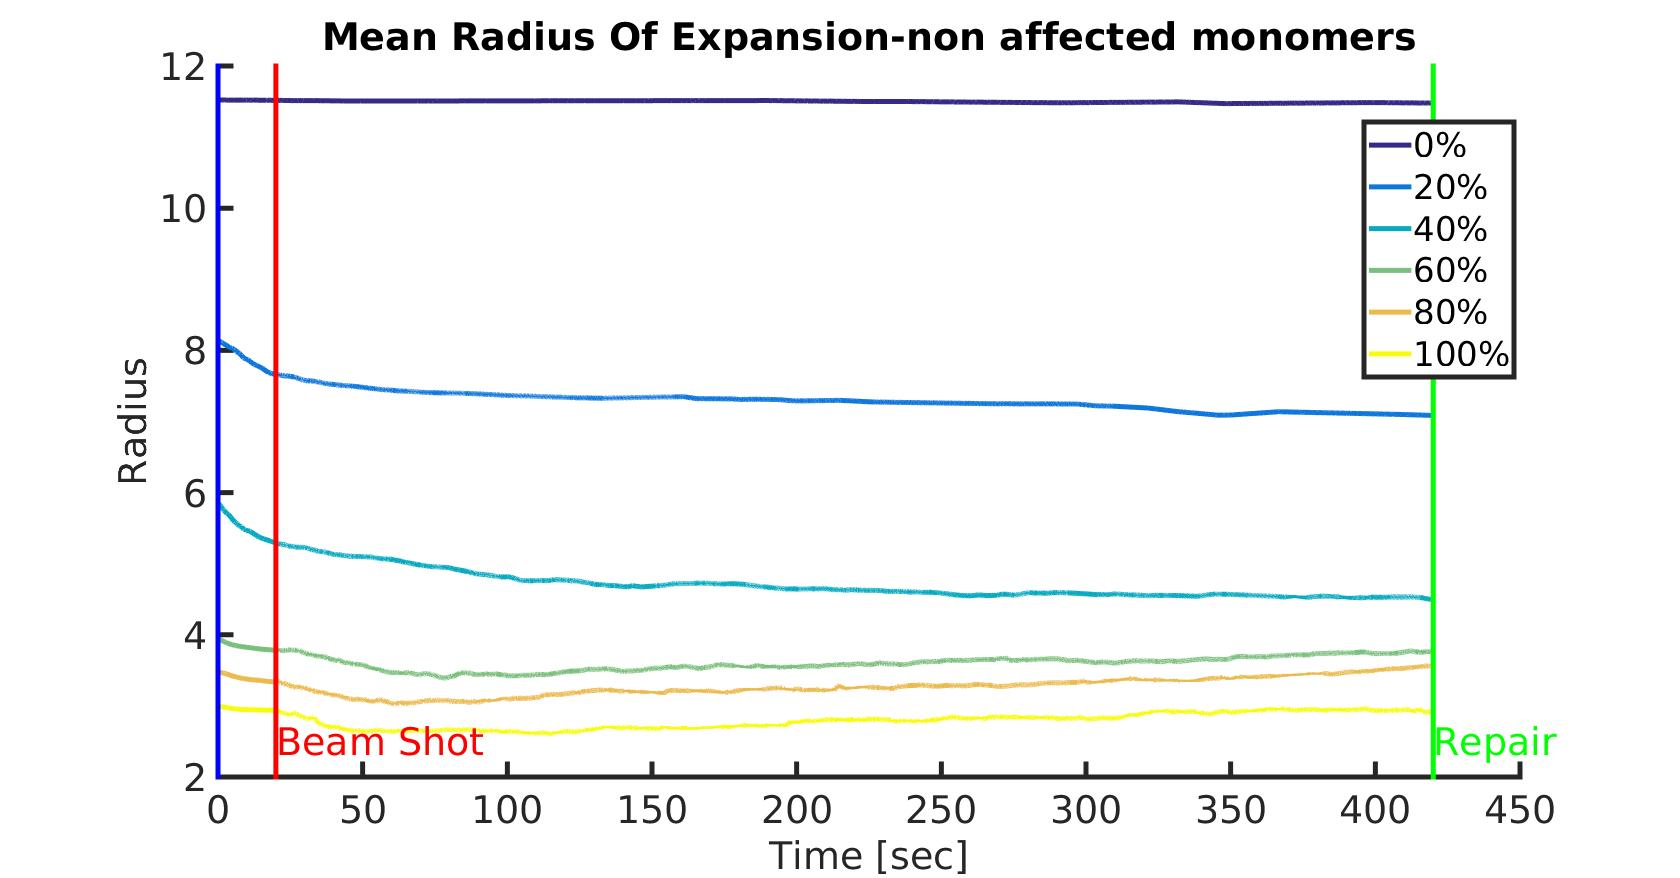
\includegraphics[width=0.5\linewidth]{Images/expandNonDamaged/NoCrosslinksBroken/meanRadiusOfExpansionNonAffected}
	\caption{\tiny{\textbf{Mean radius of expansion for the damaged (left) and undamaged (right) monomers. No cross-link is broken after UVC. The expansion of the damaged monomers is equivalent to that off the non-damaged.}}}
	\label{fig:meanRadiusOfExpansionBendingNonAffecteNoBrokenCrosslinks}
	\end{figure}
	In terms of the loss of monomers in the ROI, we have:
	
	\begin{figure}[H]
	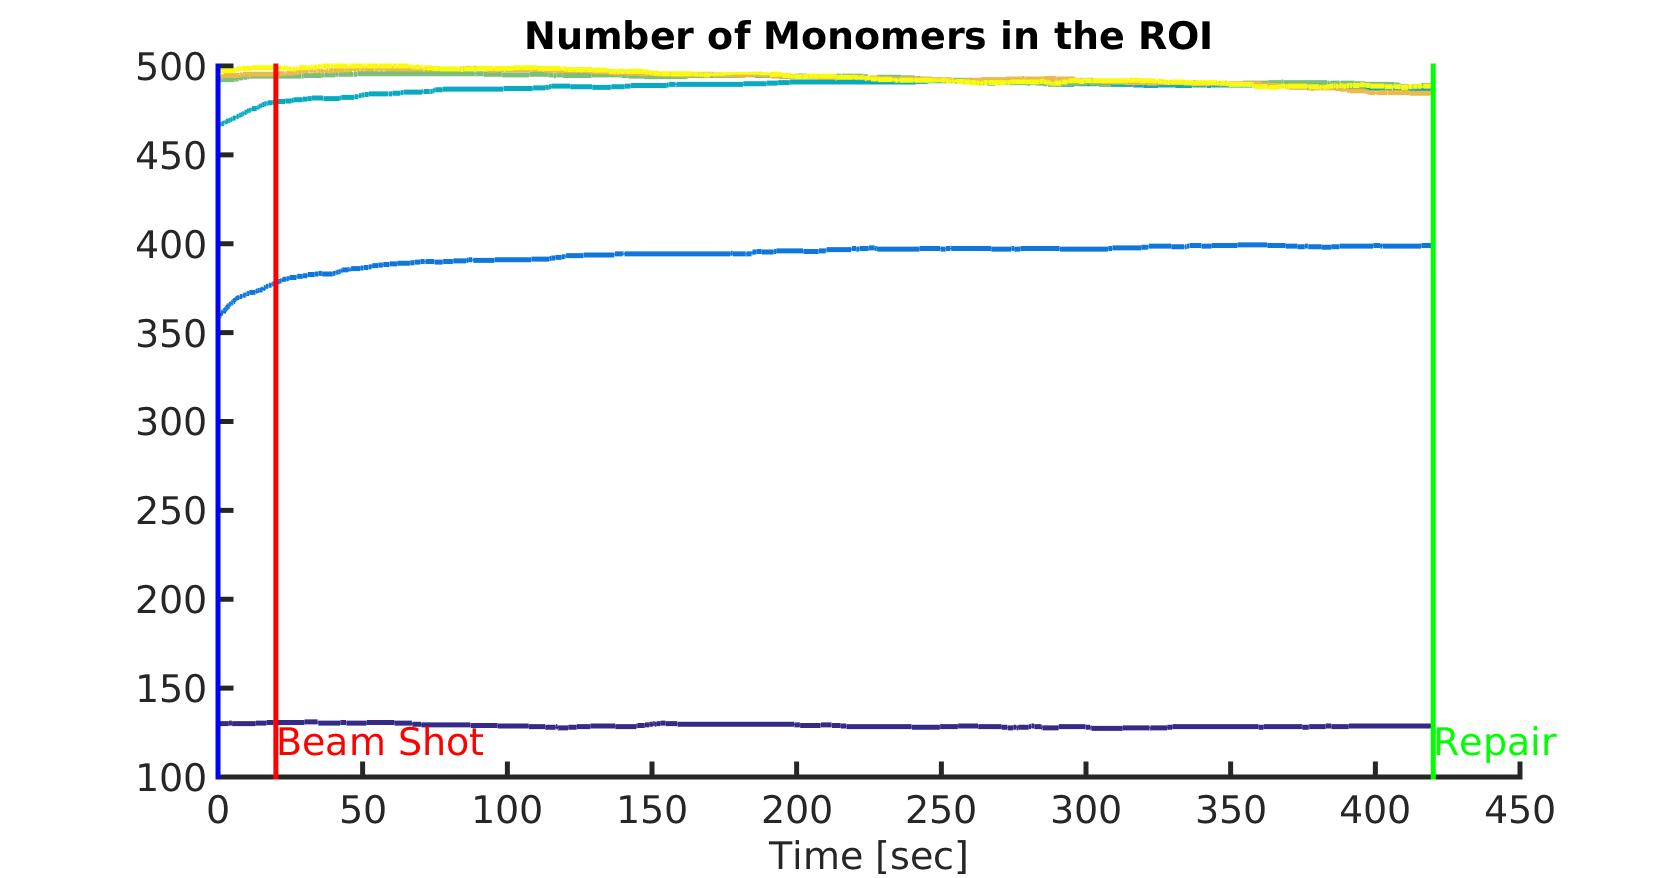
\includegraphics[width=0.5\linewidth, height=0.3\textheight]{Images/expandNonDamaged/NoCrosslinksBroken/meanNumMonomersInROI}
	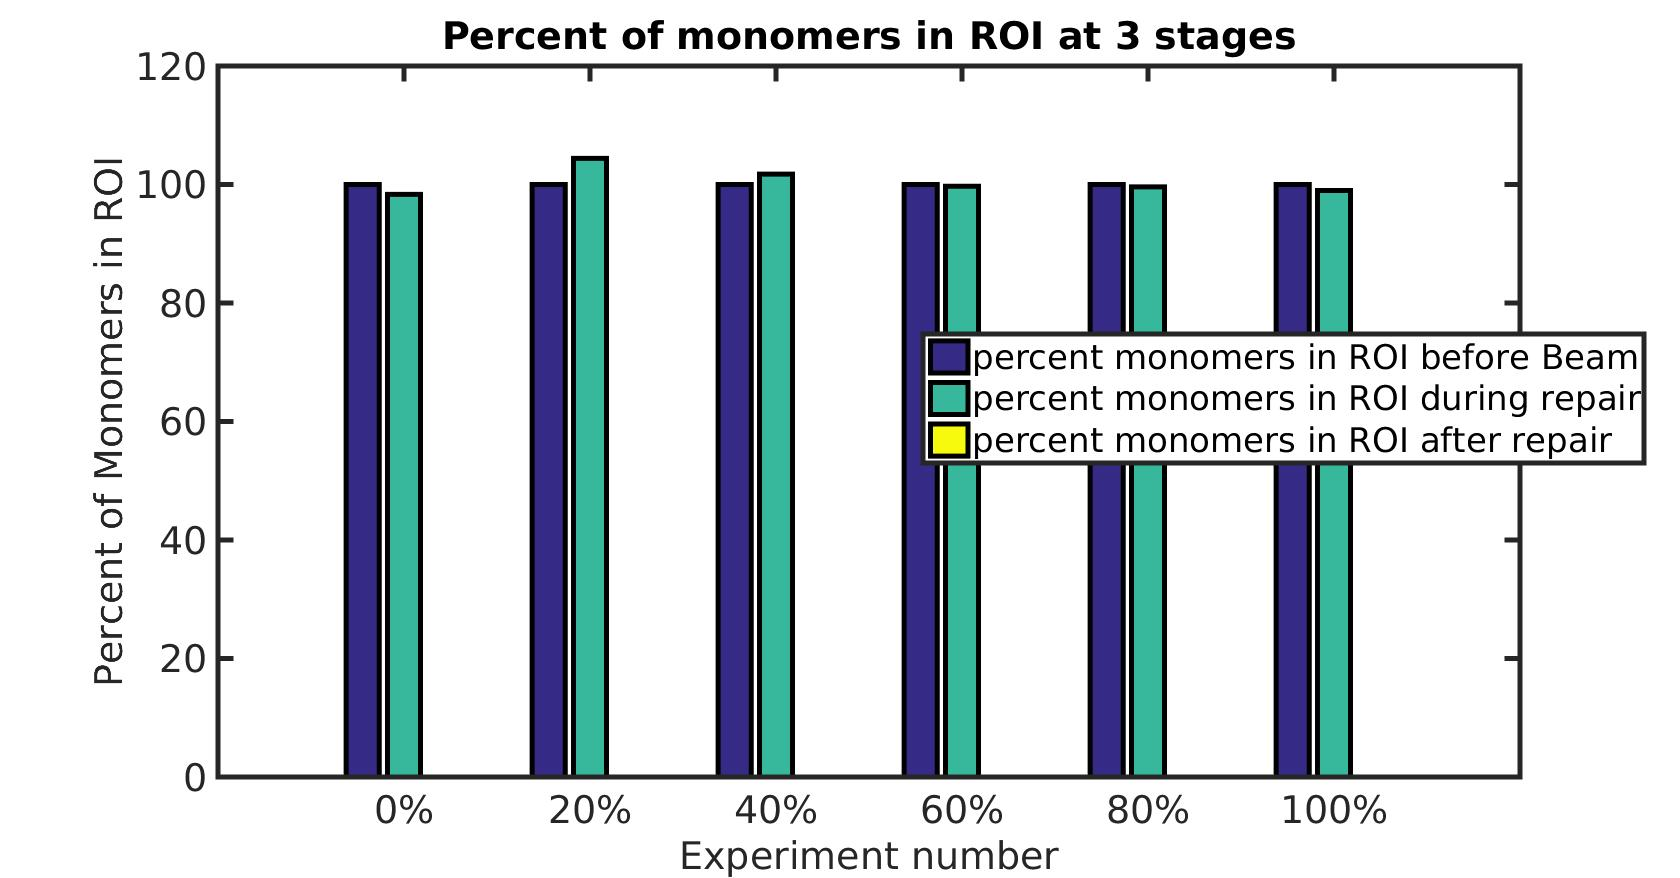
\includegraphics[width=0.5\linewidth, height=0.3\textheight]{Images/expandNonDamaged/NoCrosslinksBroken/percentageOfMonomersInROI}
	\caption{}
	\label{fig:meanNumMonomersInROINoBrokenCrosslinks}
	\end{figure}
    As can be seen in Figure \ref{fig:meanRadiusOfExpansionBendingNonAffecteNoBrokenCrosslinks}, the expansion of the damaged monomers is not stopped and it reaches that of the undamaged ones. The percentage of loss is accordingly small, since no monomers have left the ROI, which is determined by the damaged monomers radius of expansion. 
    
    
	\subsection{Assign bending to non-damaged monomers in the UVC beam}	
	 To simulate the process in which the repair mechanism proteins are recruited to the damage site, push away all non-damaged DNA and work on damage part, we assign bending elasticity force to monomers located within the damage region (beam) but those that were unaffected by the beam.
	 \subsubsection{Break damaged monomers' cross-links}
	 	 
	\begin{figure}[H]
	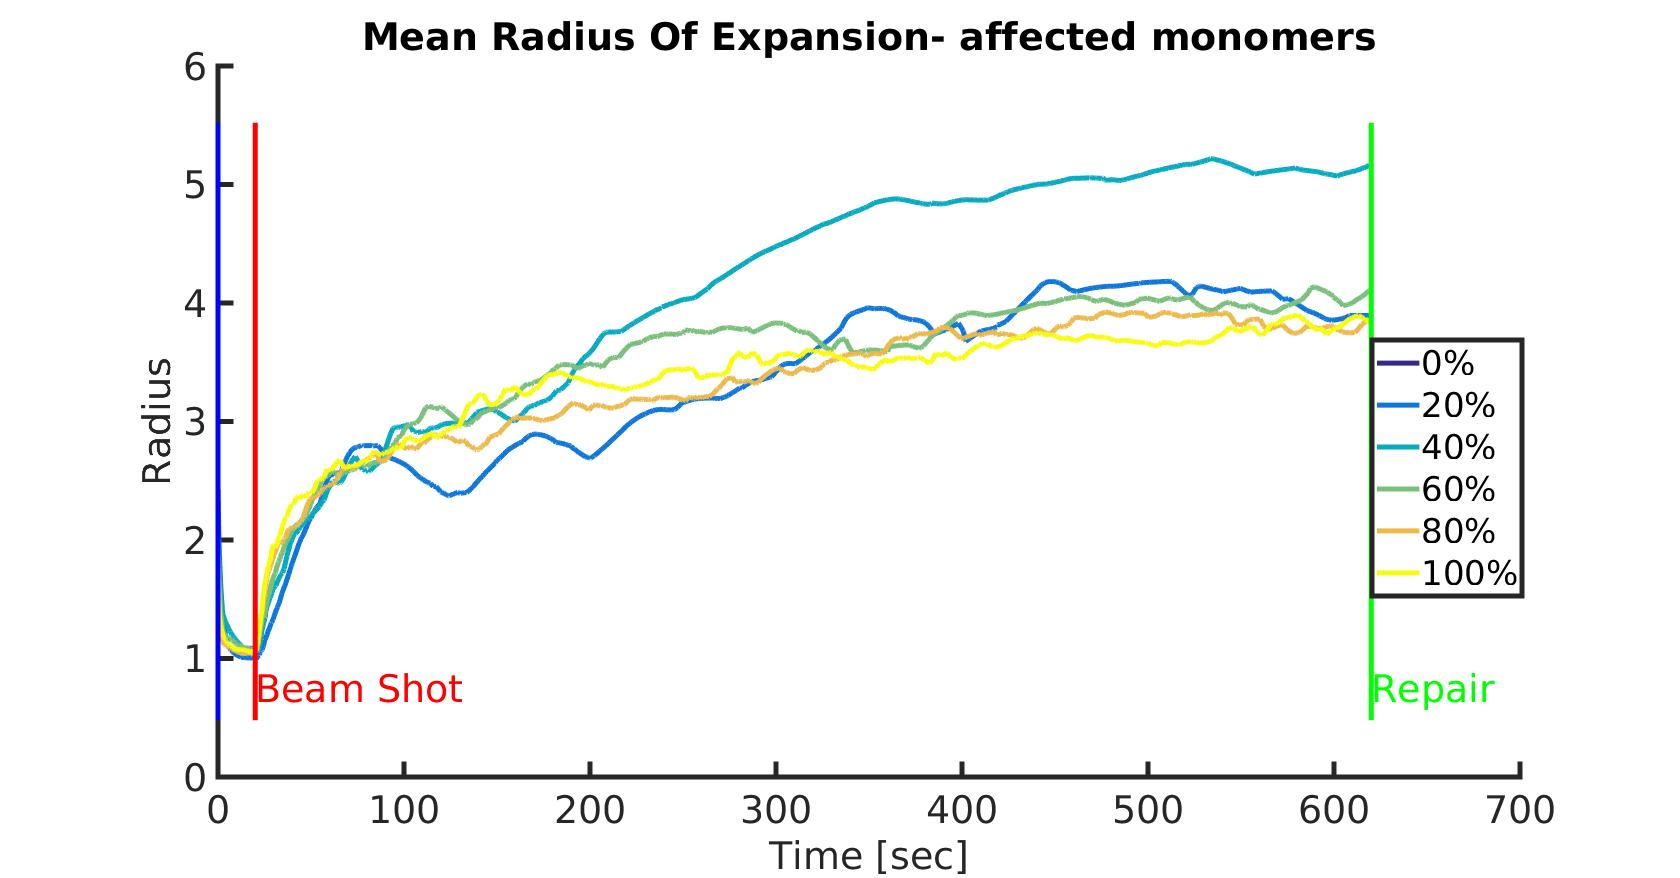
\includegraphics[width=0.5\linewidth, height=0.3\textheight]{Images/expandNonDamagedInBeam/breakDamagedCrosslinks/meanRadiusOfExpansionAffected}
	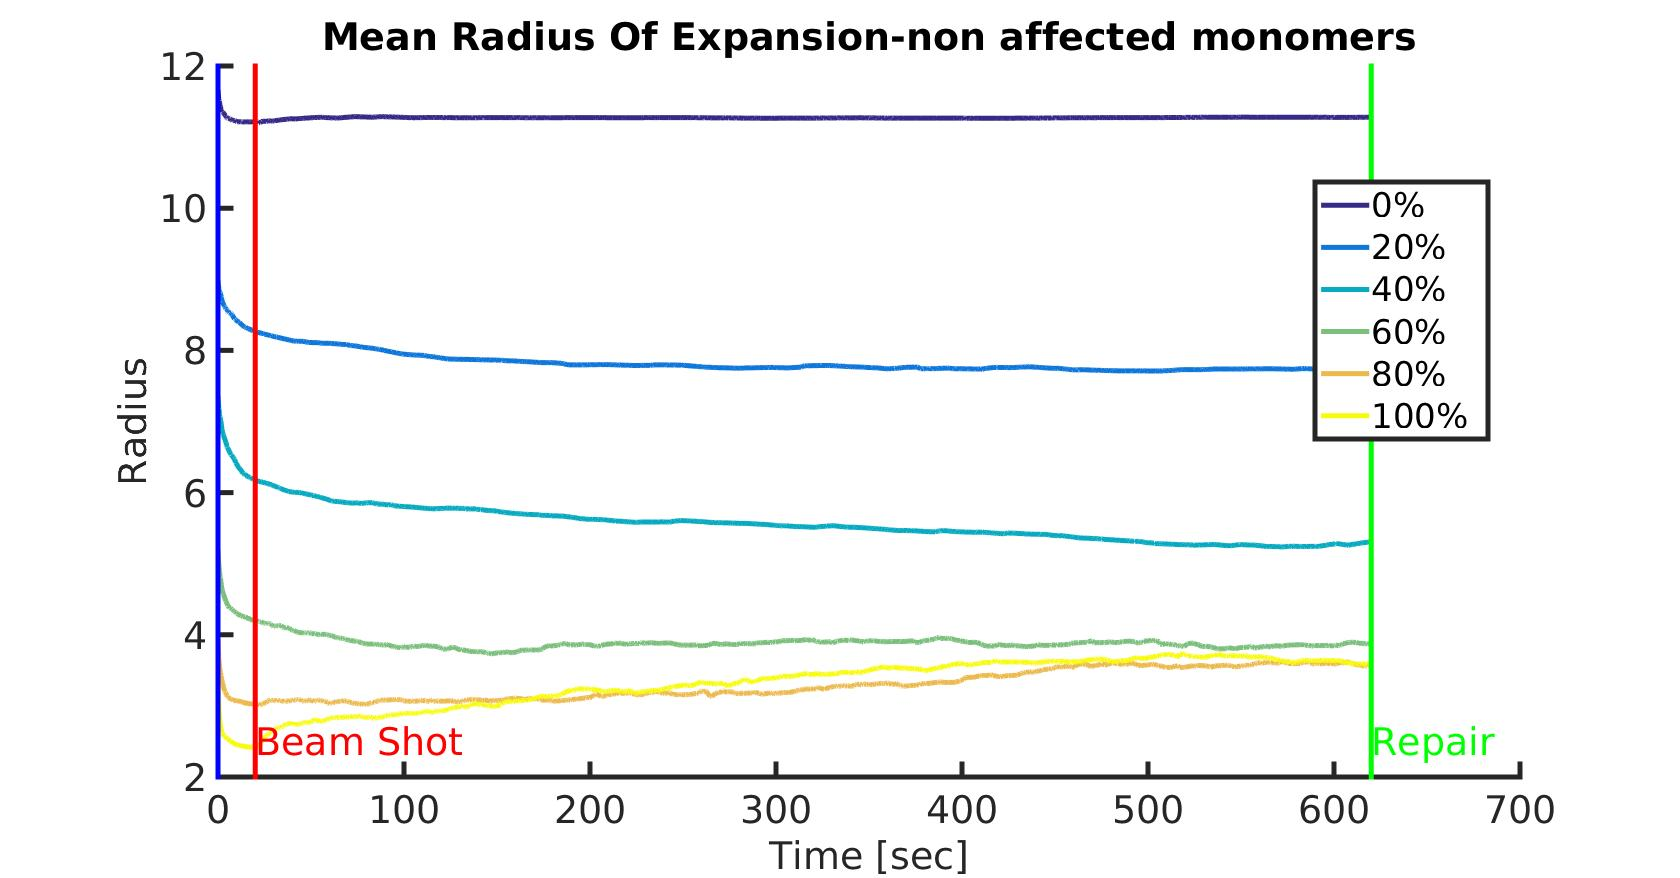
\includegraphics[width=0.5\linewidth, height=0.3\textheight]{Images/expandNonDamagedInBeam/breakDamagedCrosslinks/meanRadiusOfExpansionNonAffected}
	\caption{\tiny{\textbf{The radius of expansion for the affected (left) and the non-affected (right) monomers. The radius of the affected monomers expands roughly 3-times its initial value and converages to that of the non-affected monomers. There were non affected monomers in the case of 0\% conectivity, therefore the curve is not shown. (500 monomers, no Lennard-Jones, bending potential assigned to non-damaged monomers in the ROI)}}}
	\label{fig:meanRadiusOfExpansionAffected}
	\end{figure}
	 
	 \subsubsection{Keep all cross-links after UVC}
	 [Not tested]
	 
	 
	 \subsection{Region of exclusion around damaged monomers}
	 To simulate the arrival and crowding of repair mechanism in the damage site, we apply a mechanical pushing force around each damaged monomer after UVC. This force operates in a finite range around each damaged monomers, with magnitude inversely proportional to the distance between the force's center and the monomers. multiple focus of force operates and updated simultaneously at each simulation step. Each force locus is placed on the damaged monomer. We test the expansion and DNA loss in the ROI similarly to the previous subsection. The ROI is determined according to the expansion of the damaged monomers, and we test two scenarios: one with cross-linked removed from and to the damaged monomer post UVC, and the second with all cross-links kept after UVC damage. 
     
     Description of the mechanical exclusion potential:
     \begin{equation*}
     U_m(r_i)= \frac{k_m}{2}\sum_{i,j}(R_m-|r_i-c_j|)^2 (H(0)-H(R_m)
     \end{equation*}
     where $R_m$ is the radius of force operation- above which the force zeros-out, $c_j$ is the $j^{th}$ force center, and $r_i$ is the position of the $i^{th}$ monomer. The function $H(x)$ is the Heaviside function.
     
     The force acting on monomers at each step as a result of the mechanical exclusion potential is given by 
     \begin{equation*}
     F_m=\frac{\partial U_m}{\partial r_i}=[unfinished]
     \end{equation*}               
     
	 \subsubsection{Break damaged monomers' cross-links}
	 When we break the cross-links to and from damaged monomers post UVC
	 
	\begin{figure}[H]
	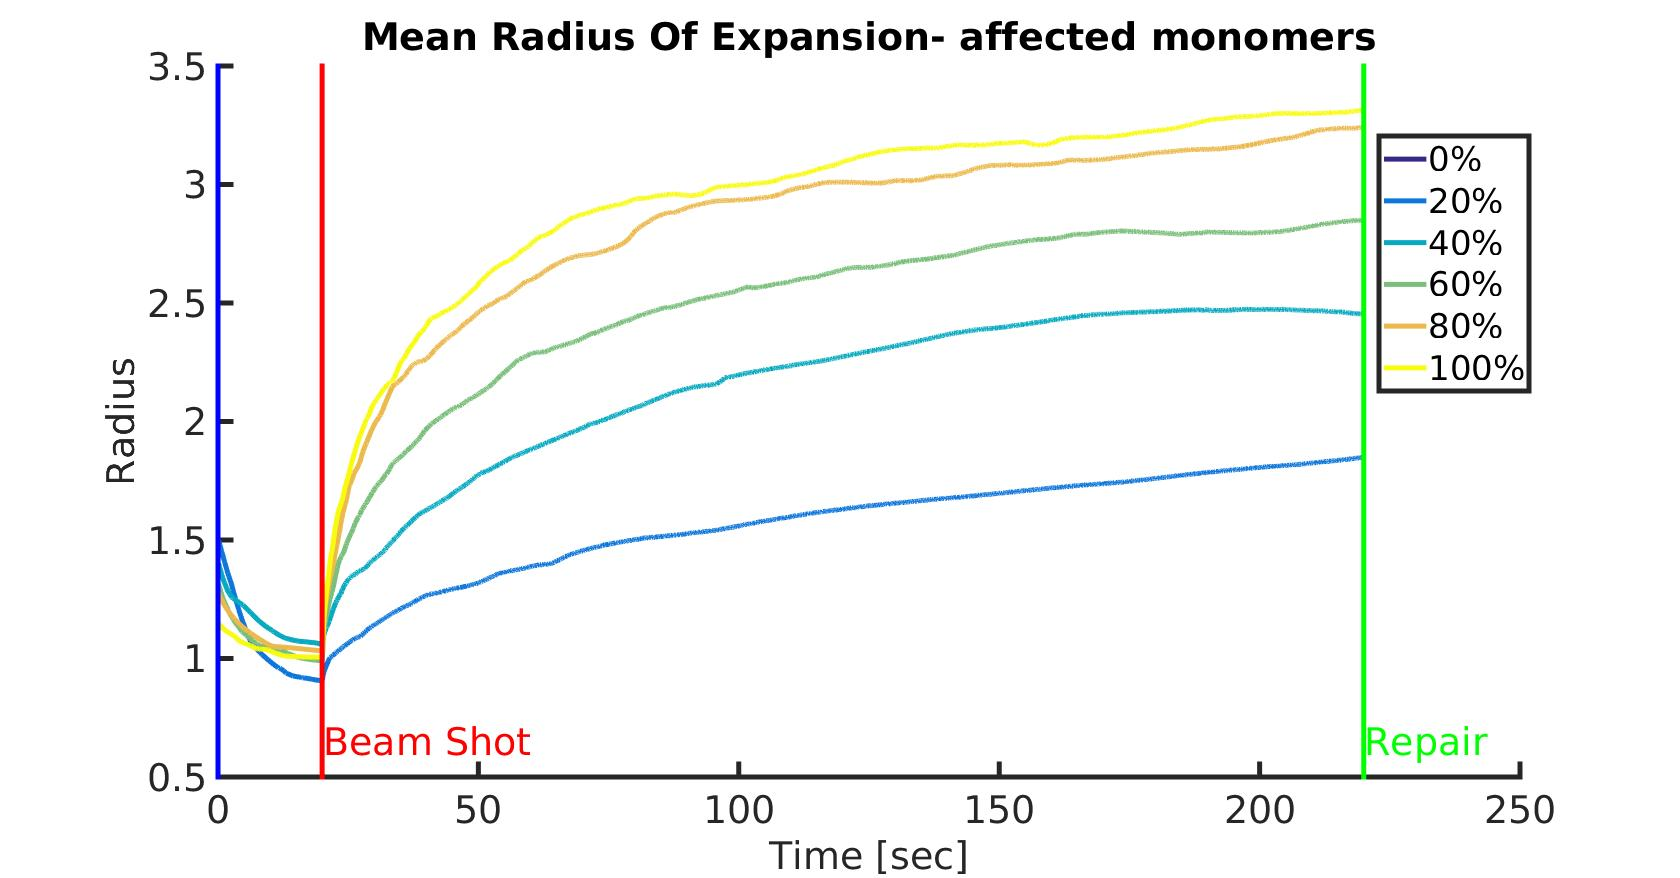
\includegraphics[width=0.5\linewidth, height=0.3\textheight]{Images/ExludeAroundDamagedMonomers/BreakDamagedCrosslinks/00/meanRadiusOfExpansionAffected}
		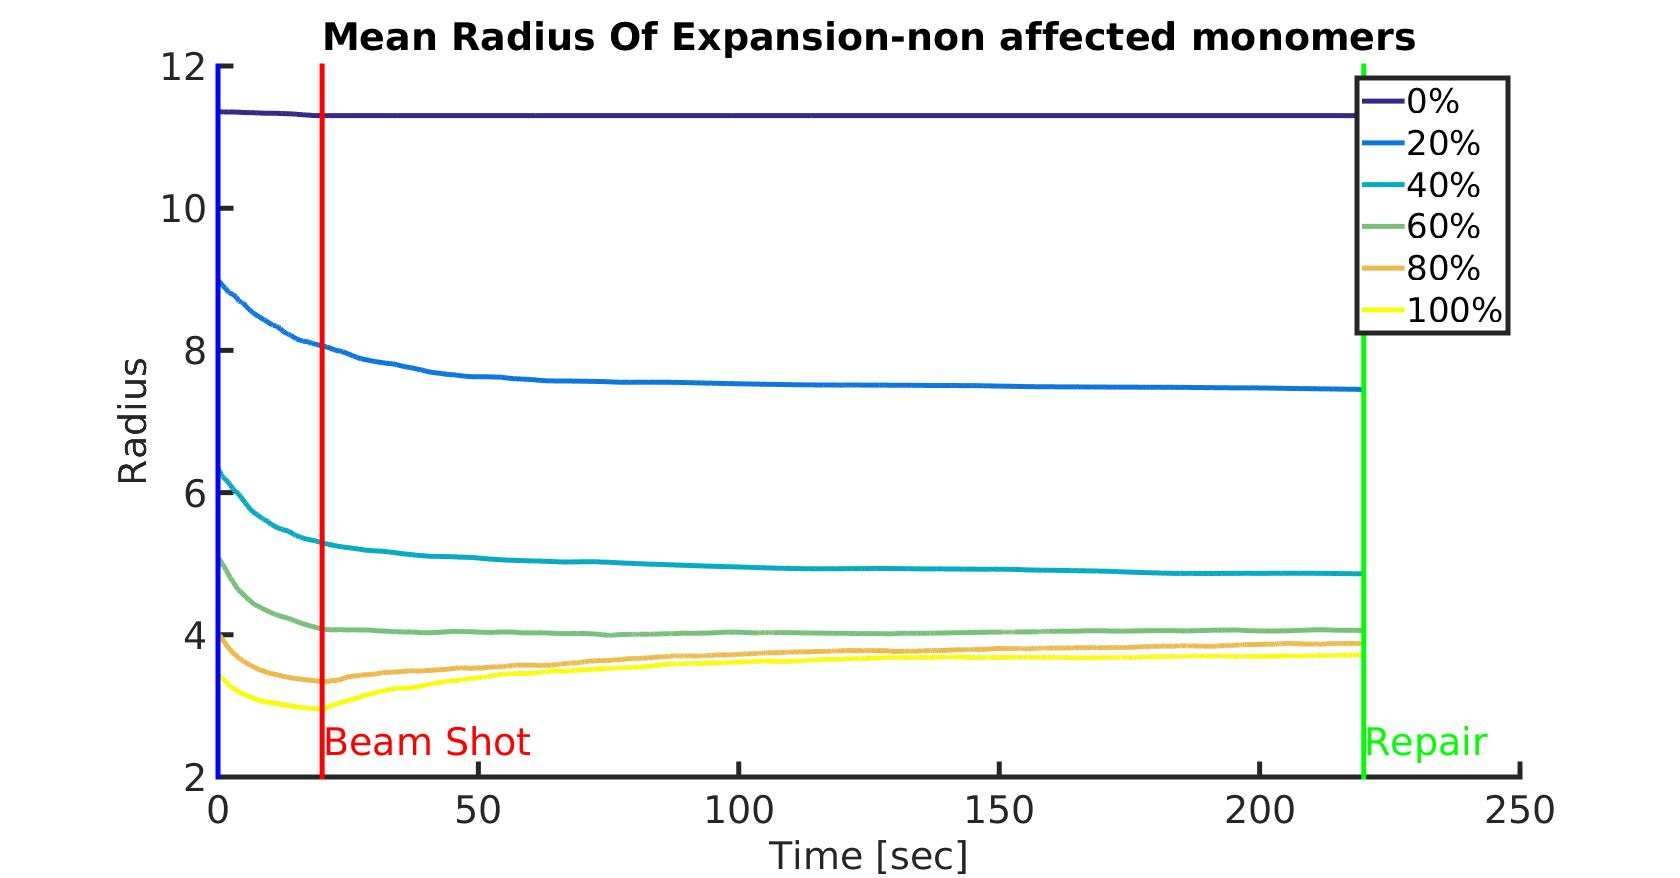
\includegraphics[width=0.5\linewidth, height=0.3\textheight]{Images/ExludeAroundDamagedMonomers/BreakDamagedCrosslinks/00/meanRadiusOfExpansionNonAffected}
	\caption{}
	\label{fig:meanRadiusOfExpansionAffected}
	\end{figure}
	 In terms of DNA loss in the ROI
	 
	\begin{figure}
	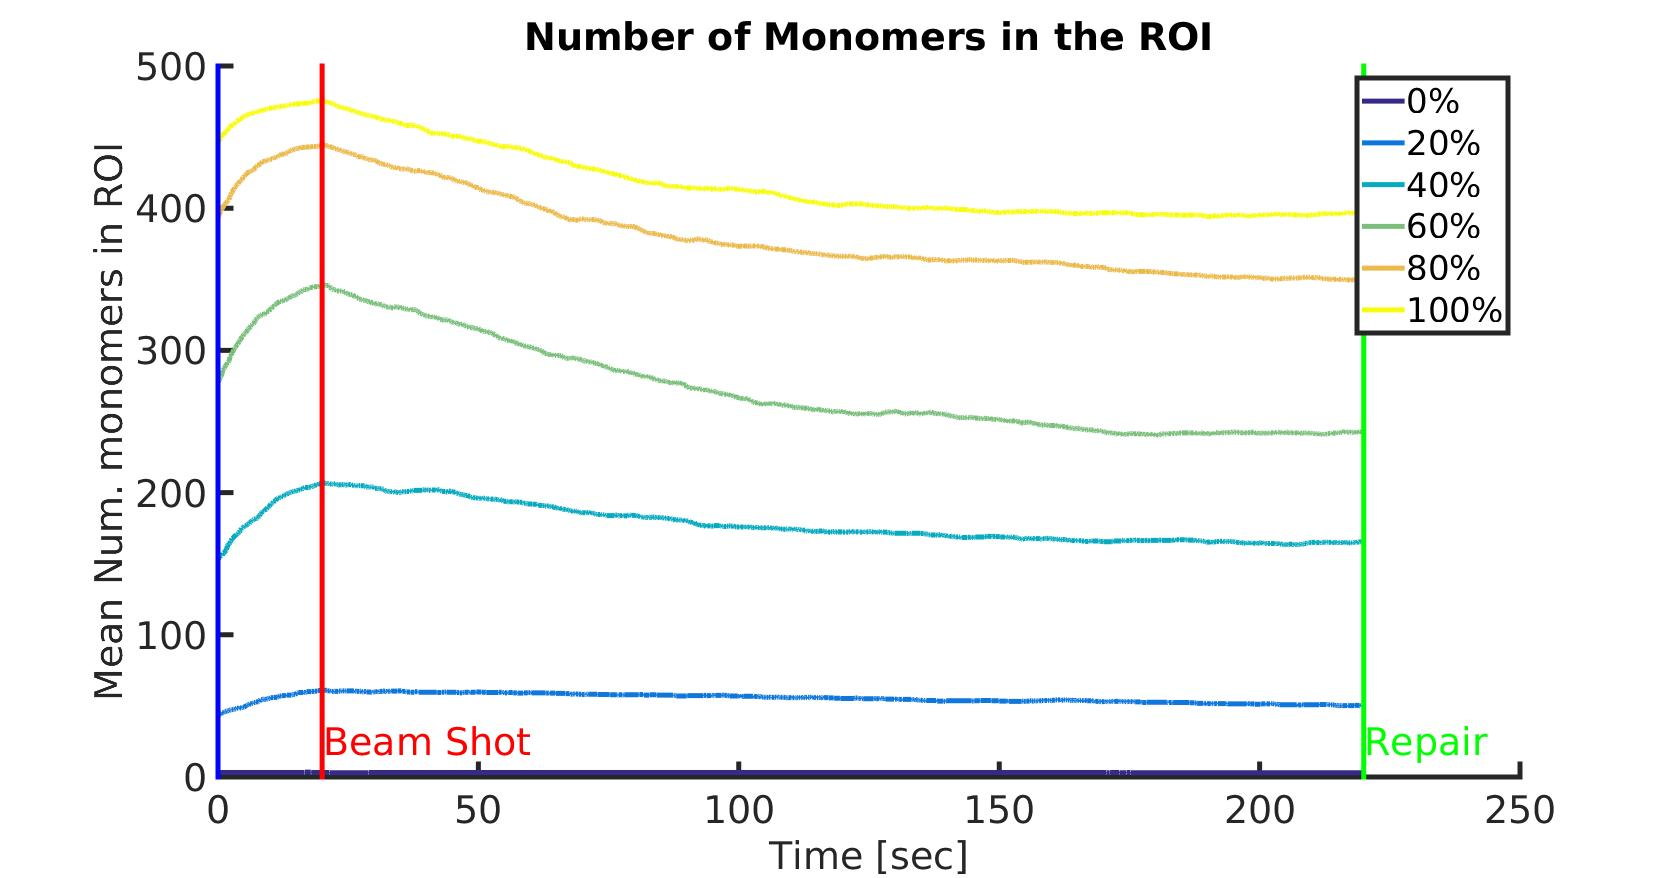
\includegraphics[width=0.5\linewidth, height=0.3\textheight]{Images/ExludeAroundDamagedMonomers/BreakDamagedCrosslinks/00/meanNumberOfMonomersInROI}
		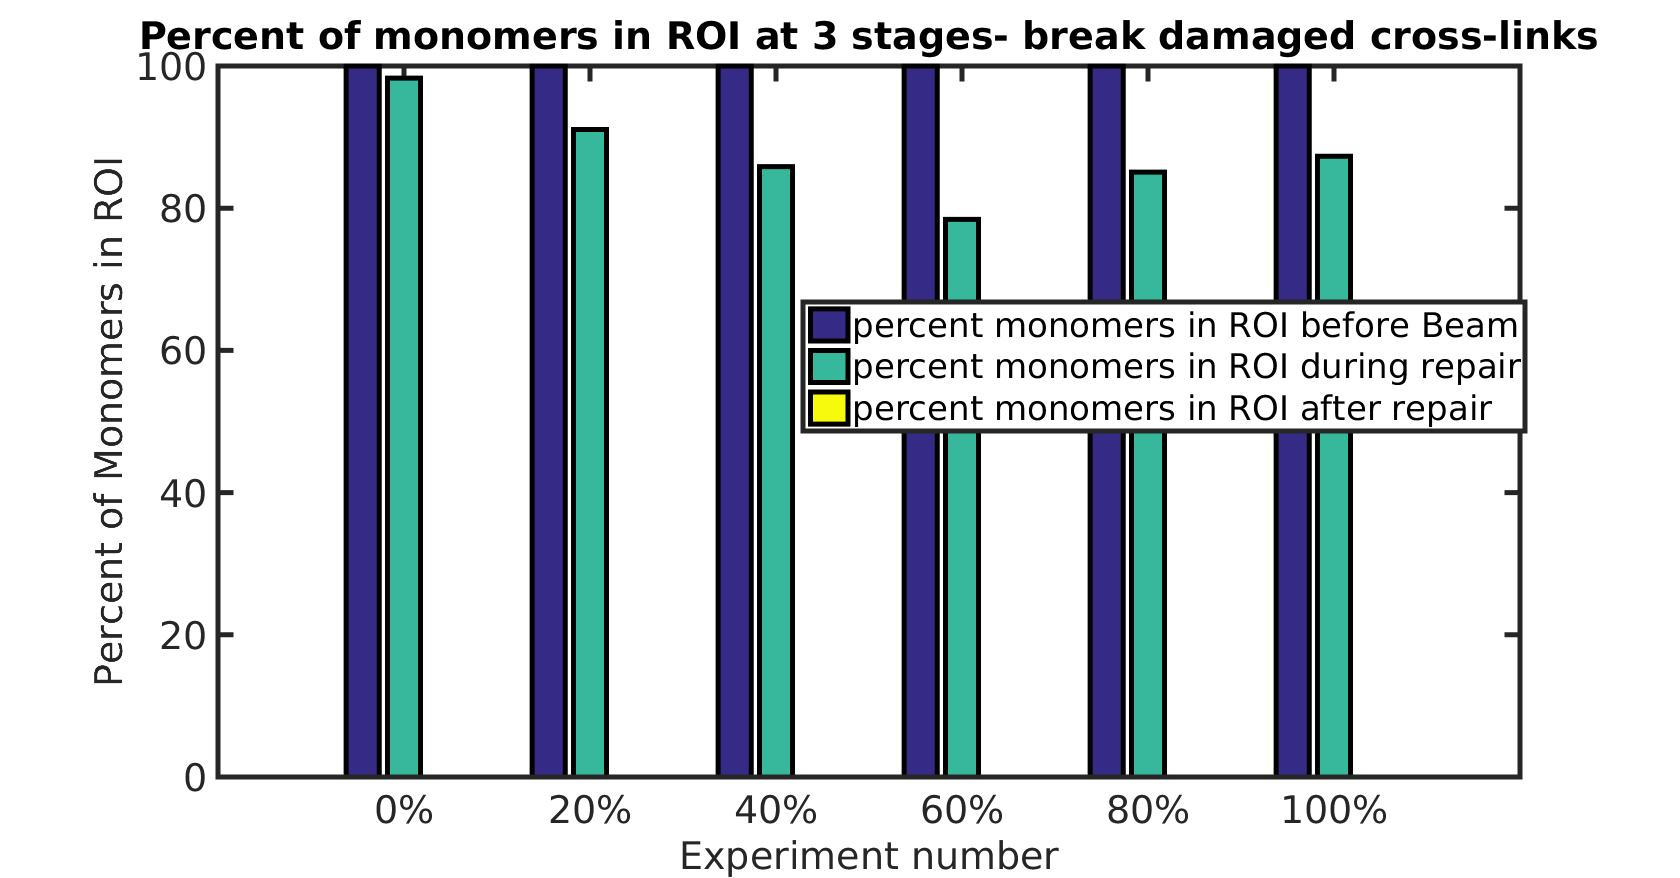
\includegraphics[width=0.5\linewidth, height=0.3\textheight]{Images/ExludeAroundDamagedMonomers/BreakDamagedCrosslinks/00/percentOfMonomersInROI}
	\caption{}
	\label{fig:meanNumberOfMonomersInROI}
	\end{figure}
	 
	 
	 \subsubsection{No cross-links broken}
	 When we do not break the cross-links to and from the damaged monomers post UVC, result show:
	 	 
	\begin{figure}[H]
	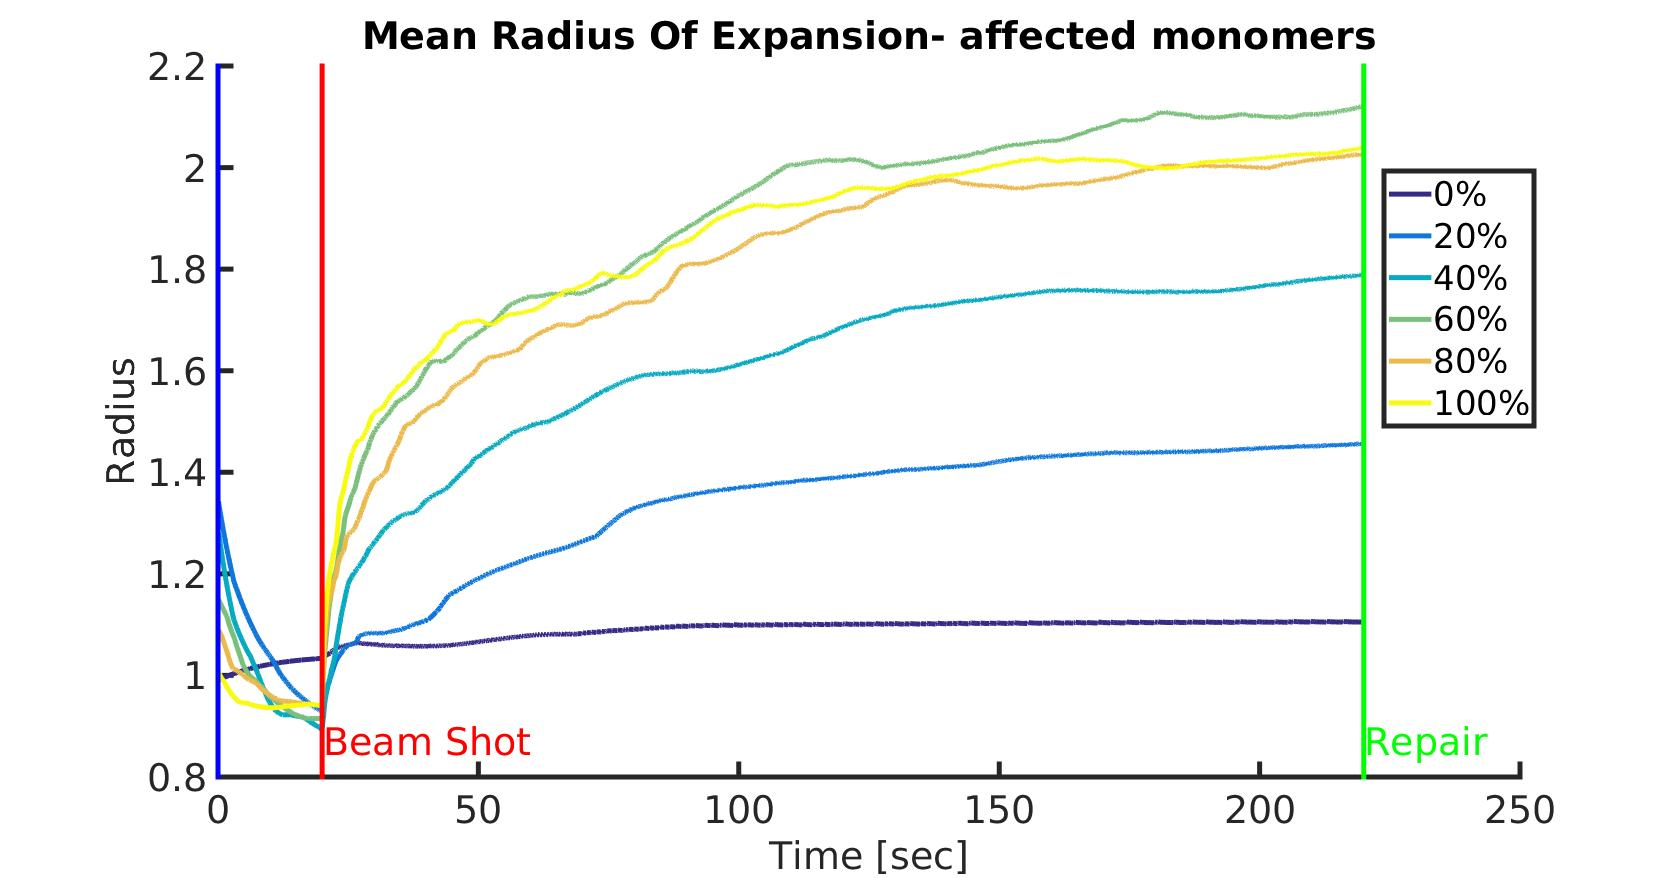
\includegraphics[width=0.5\linewidth, height=0.3\textheight]{Images/ExludeAroundDamagedMonomers/NoCrosslinksBroken/00/meanRadiusOfExpanssionAffected}
	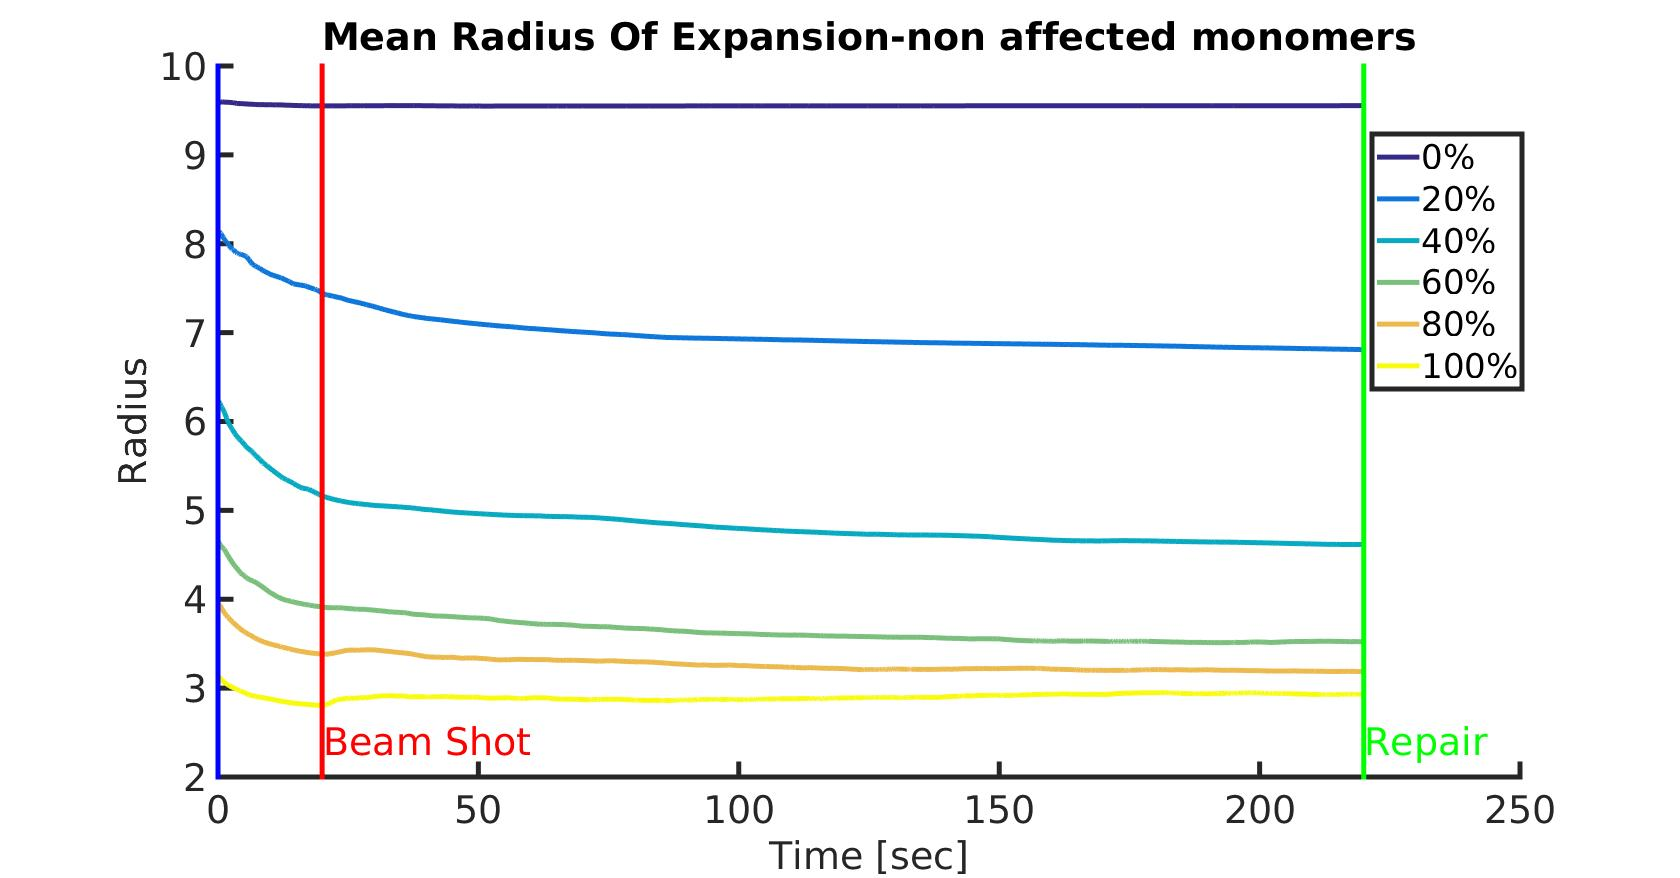
\includegraphics[width=0.5\linewidth, height=0.3\textheight]{Images/ExludeAroundDamagedMonomers/NoCrosslinksBroken/00/meanRadiusOfExpanssionNonAffected}
	\caption{\tiny{\textbf{The mean radius of expansion for the damaged (left) and non-damaged (right) monomers for different percentage of cross-linking. Post UVC a circle of exclusion is drawn around the position of each damaged monomers and a pushing force is applied to all monomers located within the circle. . this force serves to simulated the recruit and crowding of the repair mechanism at the damage site. The radius of expansion of the damaged monomes converges for all percentages of cross-linking and never exceeds those of the non-damaged.in all cases, the expansion converges to roughly twice that of the initial radius of expansion at UVC initiation. (400 monomers. No Lennard-Jones, no bending potential, all cross-links are kept post UVC)}}}
	\label{fig:meanRadiusOfExpanssionAfected}
	\end{figure}
	
	In terms of the DNA loss, we get 
	
	\begin{figure}[H]
	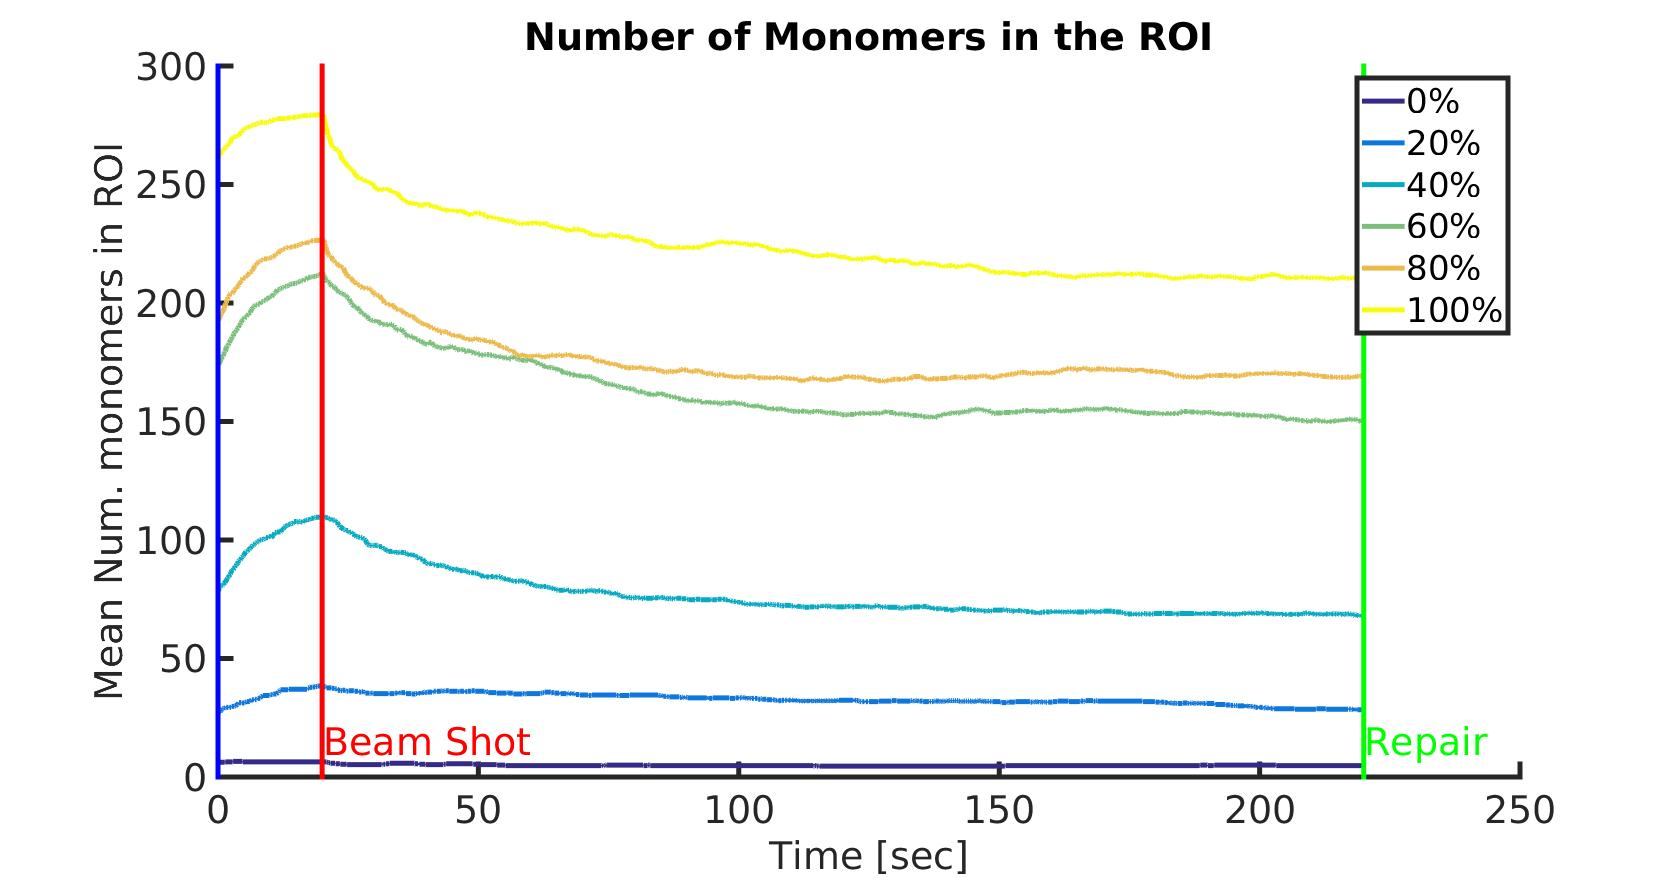
\includegraphics[width=0.5\linewidth, height=0.3\textheight]{Images/ExludeAroundDamagedMonomers/NoCrosslinksBroken/00/meanNumMonomersInROI}
	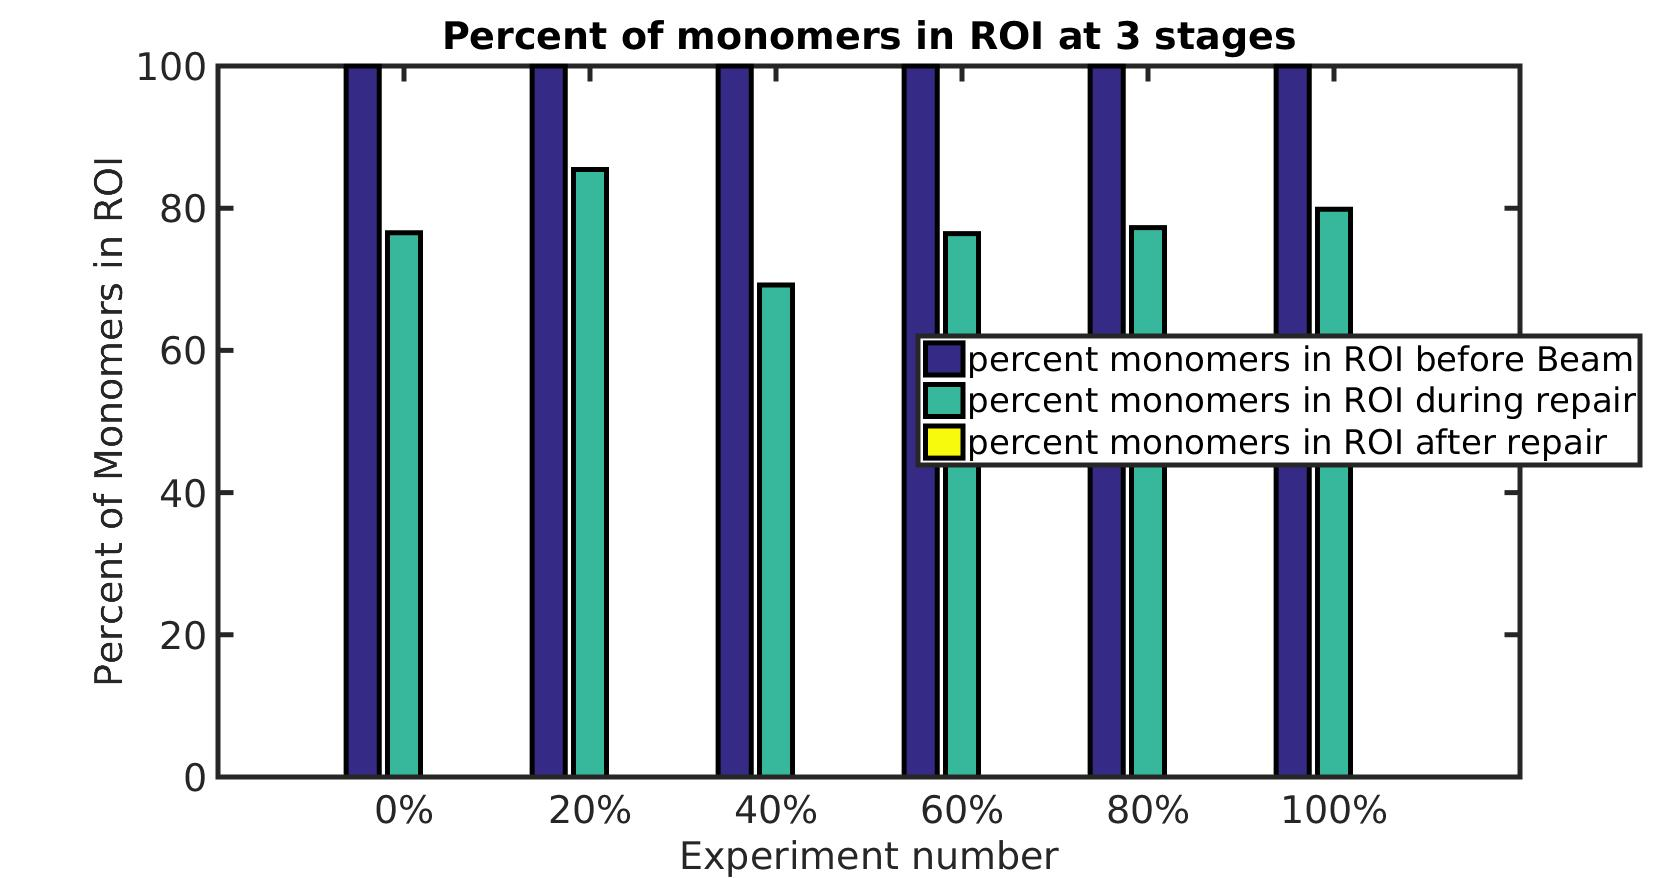
\includegraphics[width=0.5\linewidth, height=0.3\textheight]{Images/ExludeAroundDamagedMonomers/NoCrosslinksBroken/00/percentOfMonomersInROI}
	\caption{\tiny{\textbf{The absolute number of monomers in the ROI (left) and the percentage of loss at the end of simulation (right). For low degree of connectivty we have little to no change in the number of monomers in the ROI. Low level of conectivity turns out to be less reliable due to the fact that initialy less monomes are located near the center of mass of the polymer, where the beam is shot through. For high degree of connectivity (60-100\%, we see decrease roughly around 20\%. (400 monomers. No Lennard-Jones, exclusion around damaged monomers. no bending potential. All cross-links are kept post UVC)) }}}
	\label{fig:meanNumMonomersInROIExclusionAroundDamaged}
	\end{figure}

	 \subsection{Conclusions}
	 We have examined several scenarios in which a UVC beam is shot towards the center-of-mass of a polymer. As a result, an expansion of the polymer is seen experimentally. To mimic the expansion of the polymer around the damage zone, we have assigned bending elasticity to either of the four groups: the affected monomers (and their nearest neighbors) the non-affected monomers, the non-affected monomers in the UVC beam, and both the affected and non-affected alike. 
     To keep the polymer from expanding, we add random cross-links between different parts of the polymer. After UVC beam was shot, we either release the cross-links or keep them all.
     
     It was shown that when bending is assigned to the damaged monomers, the expansion in the damaged monomers is larger than that of the non-damaged one. Because we determine the region of interest according to the damaged monomers' radius of expansion, it then shows immediately that there could be no loss of monomers in the region, since it include most of them (bot damaged and non-damaged). In contrast, assigning bending to the non-damaged monomers (while keeping non-damaged cross-links) proved to supply exactly the result we have anticipated: the damaged monomers redistribute, since the cross-links are broke), the non-damaged monomers leave the ROi determined by the damaged monomers, and so allow a reduction of 20\% (if the cross-linking percentage exceeds 70\%). Assigning bending elasticity to the non-damaged can be justified by the fact that repair protein, whi enter the region after UVC damage, push aside all irrelevant (non-damage) DNA.
     
     
     
\end{document}